\documentclass[a4paper,10pt,notitlepage]{scrreprt}

\usepackage[T1]{fontenc}
\usepackage[english]{babel}
\usepackage[utf8x]{inputenc}
\usepackage{setspace}
\usepackage{subfig}
\usepackage{textcomp}
\usepackage{graphicx}
\usepackage{fixltx2e}
\usepackage{multirow}
\usepackage{array}
\usepackage{amssymb}
\usepackage{amsmath}
\usepackage{subfig}
\usepackage{nomencl}
\usepackage[pdfborder={0 0 0}]{hyperref}
\usepackage{natbib}
% \usepackage{makeidx}
\usepackage{nicefrac}
\usepackage{bbold}

\captionsetup{labelfont=footnotesize,textfont=footnotesize}

\newcolumntype{x}[1]{>{\begin{flushleft}$}p{#1}<{$\end{flushleft}}}
\newcolumntype{y}[1]{>{\begin{center}$}p{#1}<{$\end{center}}}
\newcolumntype{z}[1]{>{\begin{flushright}$}p{#1}<{$\end{flushright}}}
\newcolumntype{m}{>{$}l<{$}}
\newcolumntype{n}{>{$}c<{$}}
\newcolumntype{o}{>{$}r<{$}}

\bibliographystyle{plain}

% Title Page
\title{Scientific Visualization\\Project I}
\author{Milian Wolff}


\begin{document}
\maketitle

\begin{abstract}
In the first project for the scientific visualization class by Eugene Zhang I
got some first hand experience in 3D visualization algorithms, Java programming
and JavaView. While the former was very interesting and gave many opportunities
to play with parameters, models and algorithms, the latter two I could have
done without. Especially the severe lack of up-to-date documentation for the
required beta release of JavaView along with its horrible API made me waste a
lot of time.
\end{abstract}

\begingroup
\let\clearpage\relax

\tableofcontents
\endgroup

\chapter{Euler Characteristics}

The relationship between the Euler characteristic $V-E+F$ and the number of
handles turns out to be

\begin{equation}
 V-E+F = 2-2H .
 \label{eq:handle-euler}
\end{equation}

This is in so far intuitive as $2$ is the Euler characteristic of a sphere, and
$0$ that of a torus. Now every time we add another handle, we can say we add a
torus - and hence decrease the Euler characteristic by two.

The code for these results can be found in the class \texttt{Ex1\_1}. When
executed, the user can select an \texttt{*.obj} file and the program will
show it's Euler characteristic as computed by JavaView's
\texttt{PgPointSet::getEulerCharacteristic()} method. It then continues to
iterate over all sibling files with the \texttt{*.obj} extension and repeats the
procedure.

\section{Sphere}

The sphere has no handles, as can be seen in fig. \ref{fig:sphere}. As such its
Euler characteristic is of course $2$.

\section{Torus}

The torus has a single handle and hence an Euler characteristic of $0$. See
also fig. \ref{fig:torus}.

\section{Bunny}

The bunny as seen in fig \ref{fig:bunny} has no handles and is thus
topologically equivalent to the sphere with an Euler characteristic of $2$.

\section{Hand}

The hand I first suspected to be handle-free. But JavaView calculated an Euler
characteristic of $0$, which made me look for a handle. And indeed, there is a
small hole between index and middle finger, which can be seen in fig.
\ref{fig:hand}.

\section{Feline}

The feline has two handles at its tail, which is equivalent to an Euler
characteristic of $-2$. See also fig. \ref{fig:feline}.

\section{Dragon}

The dragon's tail creates a handle near its end. As such it has an Euler
characteristic of $0$ and is topologically equivalent to a torus. See also fig.
\ref{fig:dragon}.

\section{Buddha}

The Buddha has the most handles of the objects provided. Its Euler
characteristic is $-10$, and as such we should find six handles in total. Five
of them are easily visible in fig. \ref{fig:buddha1} while the last one should
be seen from the rotated view in fig. \ref{fig:buddha2}.


\begin{figure}
  \centering

  \subfloat[Sphere]{ \label{fig:sphere}
    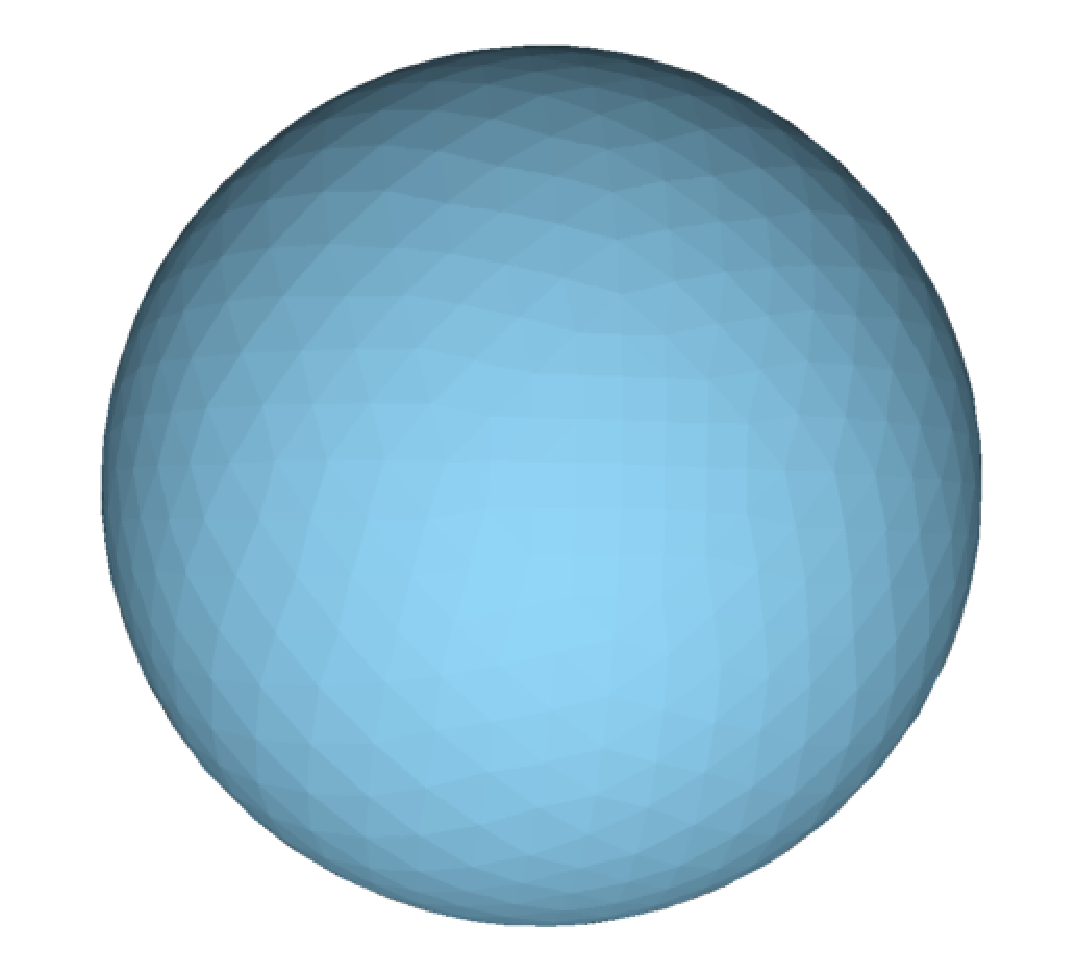
\includegraphics[scale=0.4]{sphere.eps} }
  \subfloat[Torus]{ \label{fig:torus}
    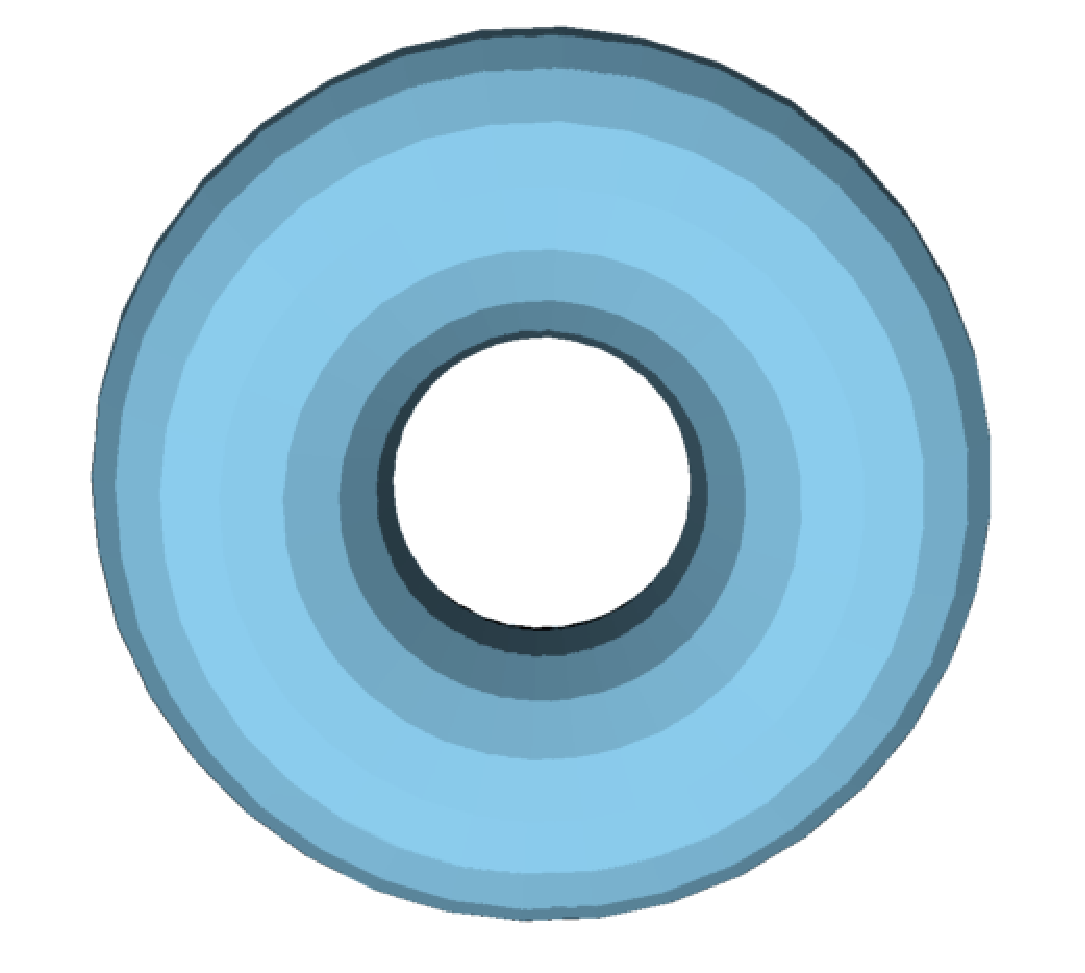
\includegraphics[scale=0.4]{torus.eps} }
  \\
  \subfloat[Bunny]{ \label{fig:bunny}
    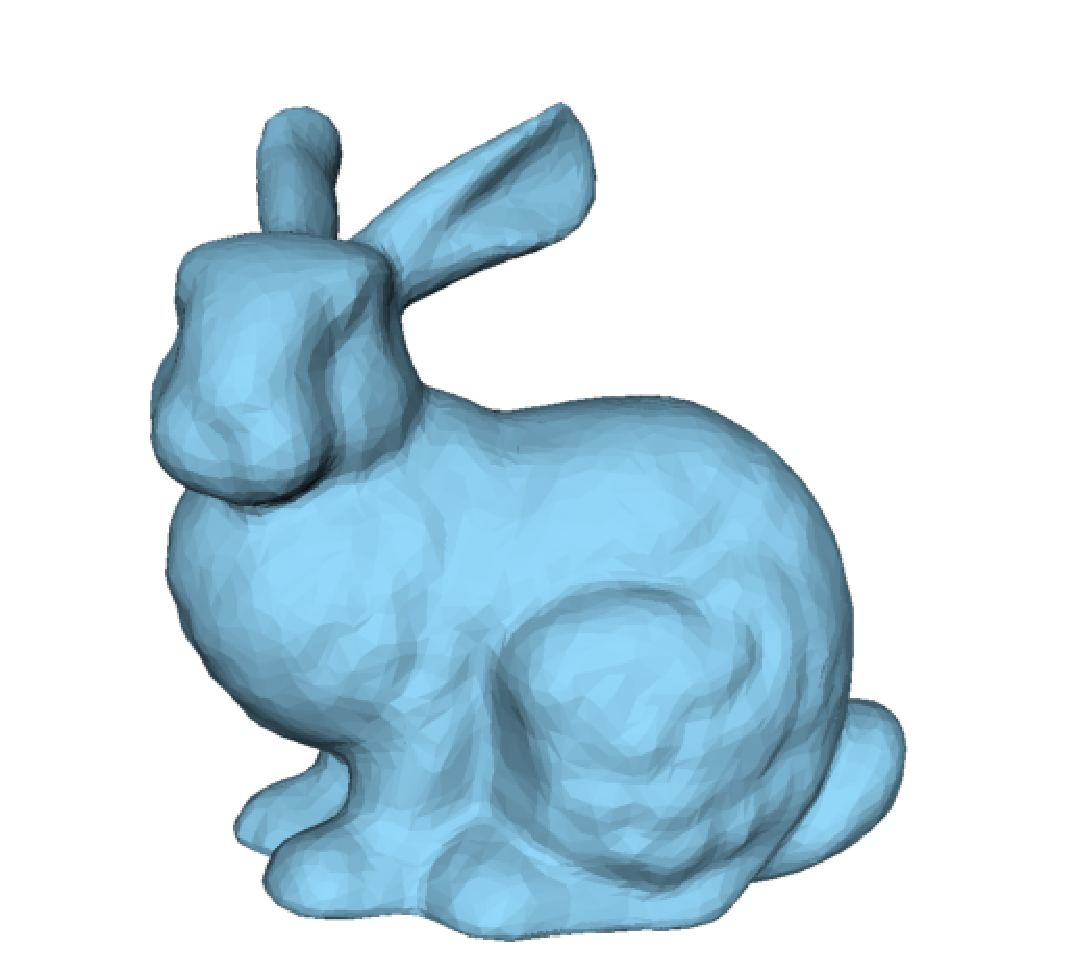
\includegraphics[scale=0.4]{bunny.eps} }
  \subfloat[Hand]{ \label{fig:hand}
    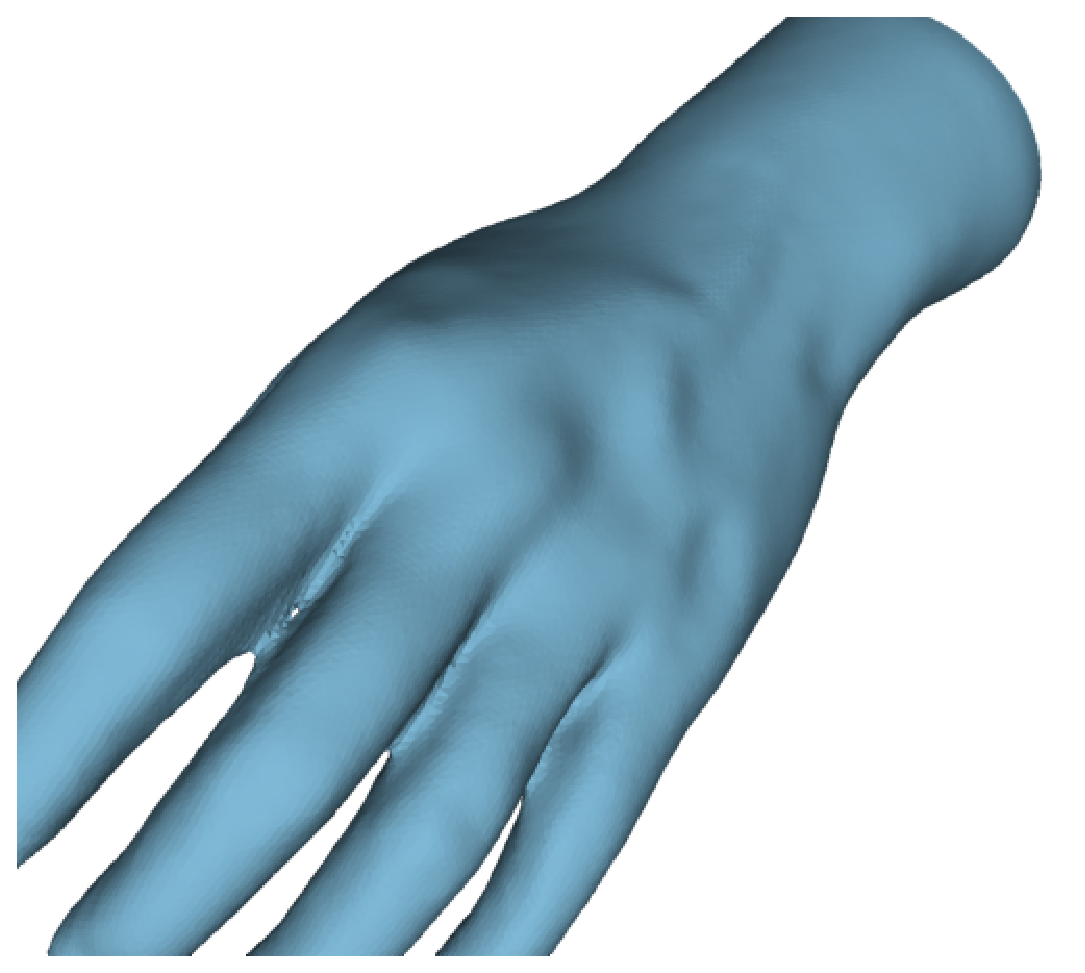
\includegraphics[scale=0.4]{hand.eps} }
  \label{fig:handles}
  \caption{Handles in Sphere, Torus, Bunny and Hand objects}
\end{figure}
\begin{figure}
  \ContinuedFloat 
  \centering
  \subfloat[Dragon]{ \label{fig:dragon}
    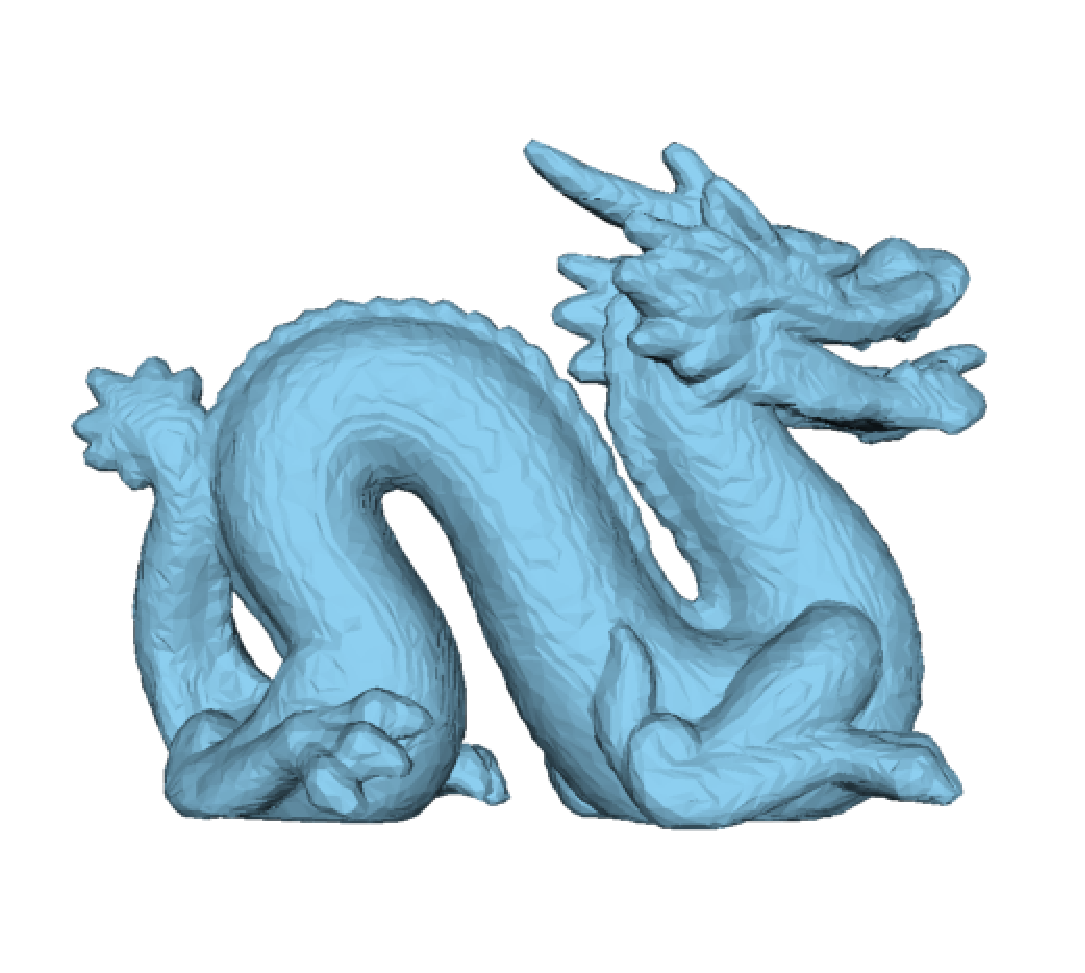
\includegraphics[scale=0.4]{dragon.eps} }
  \subfloat[Feline]{ \label{fig:feline}
    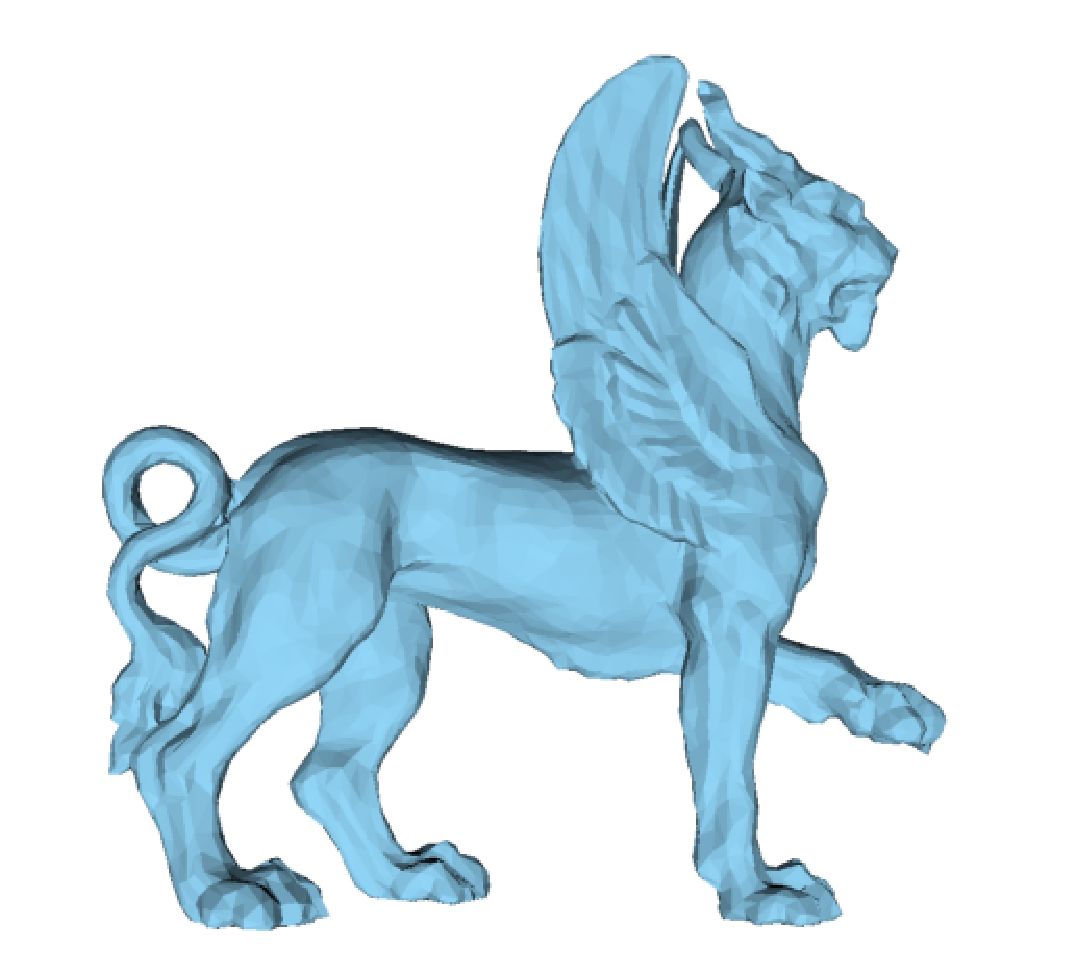
\includegraphics[scale=0.4]{feline.eps} }
  \\
  \subfloat[Buddha]{\label{fig:buddha1}
    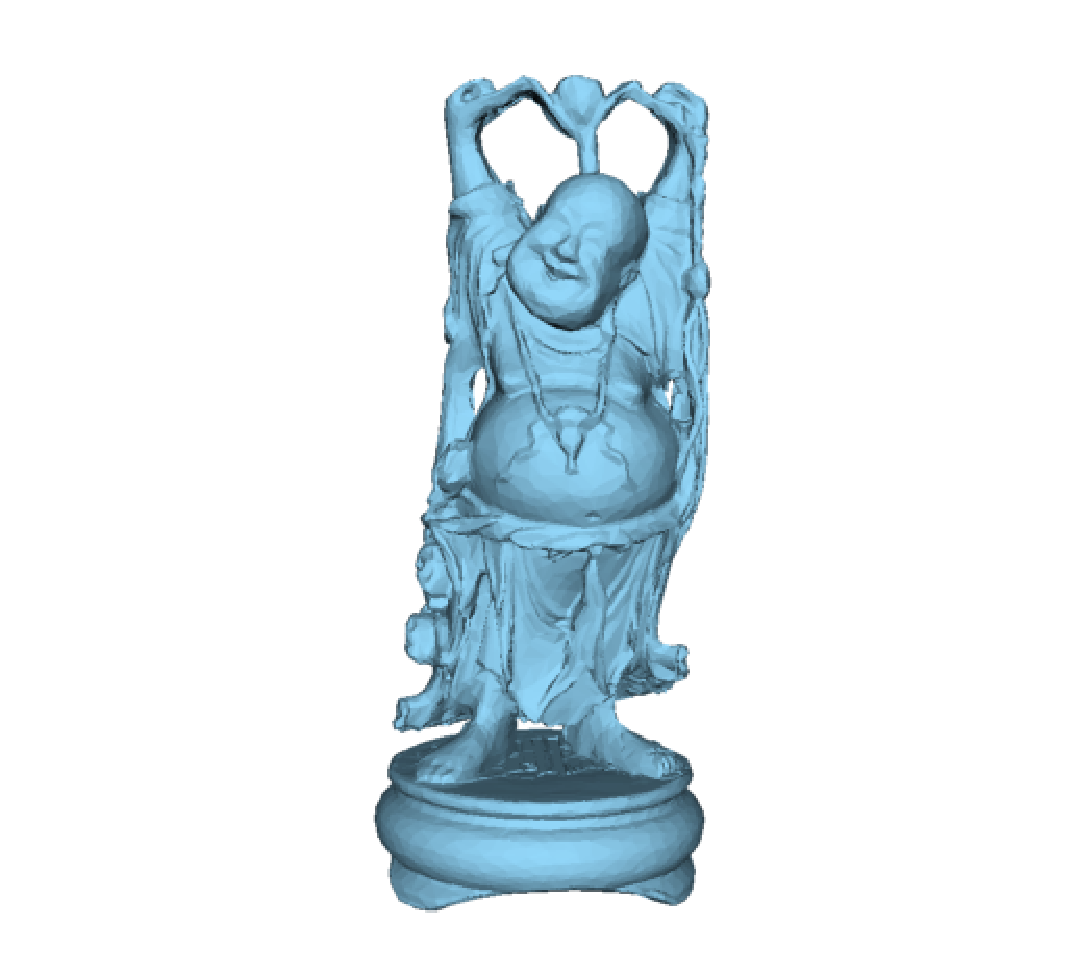
\includegraphics[scale=0.4]{budda.eps}}
  \subfloat[Buddha]{\label{fig:buddha2}
    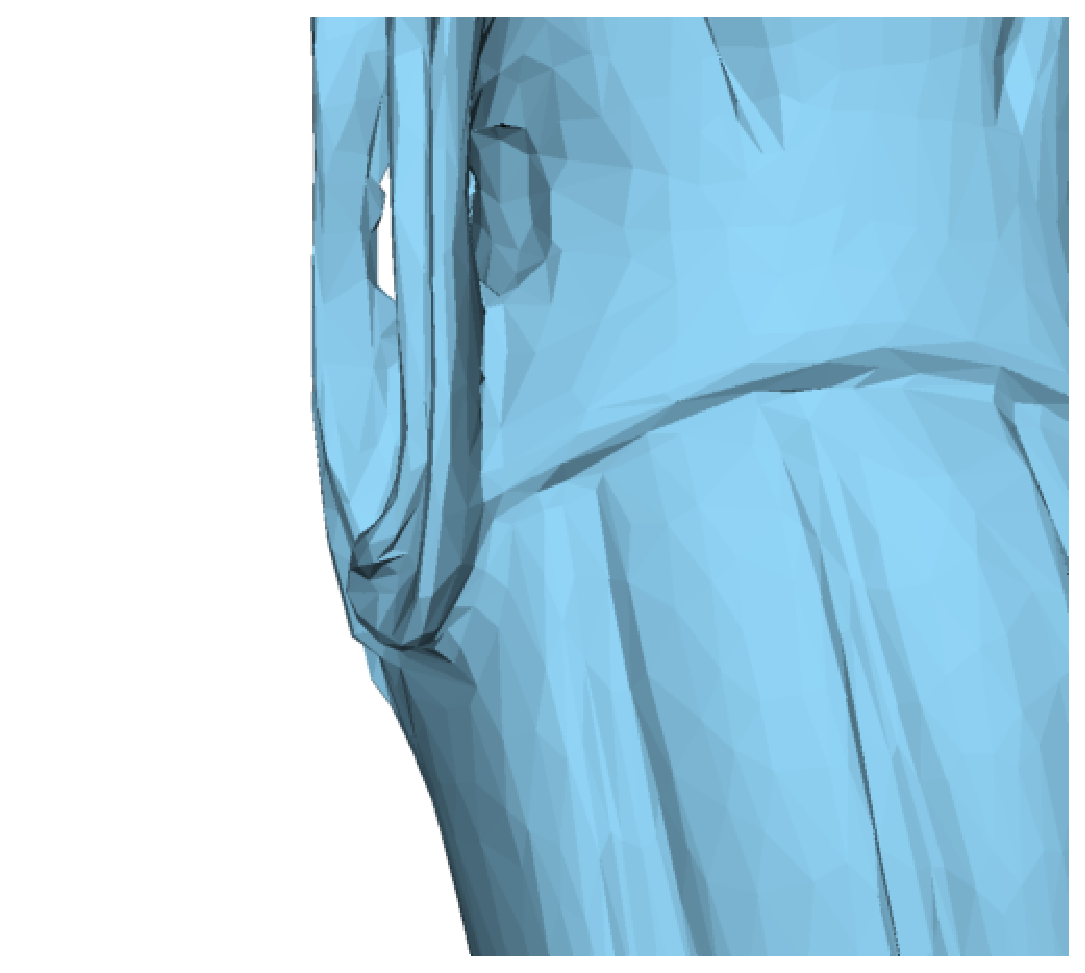
\includegraphics[scale=0.4]{budda2.eps}}

%   \label{fig:handles}
  \caption{Handles in Dragon, Feline and Buddha objects}
\end{figure}

\chapter{Mesh Coloring}

\section{Normal Mapping}

This exercise was straight forward to solve. One just iterates over the
polygons, or ``elements'' in JavaViews terminology, and assigns a color
following the equation as given on the exercise sheet:

\begin{equation}
  R = |N_x|, G = |N_y|, B = |N_z|
 \label{eq:normal-mapping}
\end{equation}

\texttt{Java.awt.Color} comes with a constructor taking three \texttt{float}
arguments. Alternatively we would multiply the absolute value with $255$ and
round off, to get an integer RGB color component value.

The results can be seen in fig. \ref{fig:bunny-normal},
\ref{fig:feline-normal}, \ref{fig:buddha-normal} and \ref{fig:dragon-normal},
and the source code is located in \texttt{Ex1\_2::setNormalMappingColors()}.

\section{3D Checkerboard}

Again, the solution to this exercise was not difficult to program. Again we map
the RGB values to $8$-bit integer values, just set the vertex colors this time.
The elements are then colored by
calling $PgElementSet::showElementFromVertexColors(true)$ on the selected
geometry.

The results can be seen in fig. \ref{fig:bunny-checker},
\ref{fig:feline-checker}, \ref{fig:buddha-checker} and
\ref{fig:dragon-checker},
and the source code is located in \texttt{Ex1\_2::set3DCheckerboardColors()}
and \texttt{Ex1\_2::f()}, while the latter combines two steps from the exercise
sheet, namely the division by $L$ followed by flooring the result and the
computation denoted by $f(n)$ on the exercise sheet.

Problems with this algorithm are the jagged edges of the single checkerboard
tiles. Especially for lower $L$ this gets worse, as can be seen in e.q. fig.
\ref{fig:dragon-checker}. This problem gets even more prominent when applying
the colorization algorithm to an Icosahedron, as seen in fig.
\ref{fig:icosahedron-checker1} and \ref{fig:icosahedron-checker2}. The reason
for both is the relatively low number of vertices compared to the size of the
polygons. If we would remesh the objects and add more points, the checkerboard
algorithm should work better again.



\begin{figure}
  \centering

  \subfloat[normal mapping]{
    \label{fig:bunny-normal}
    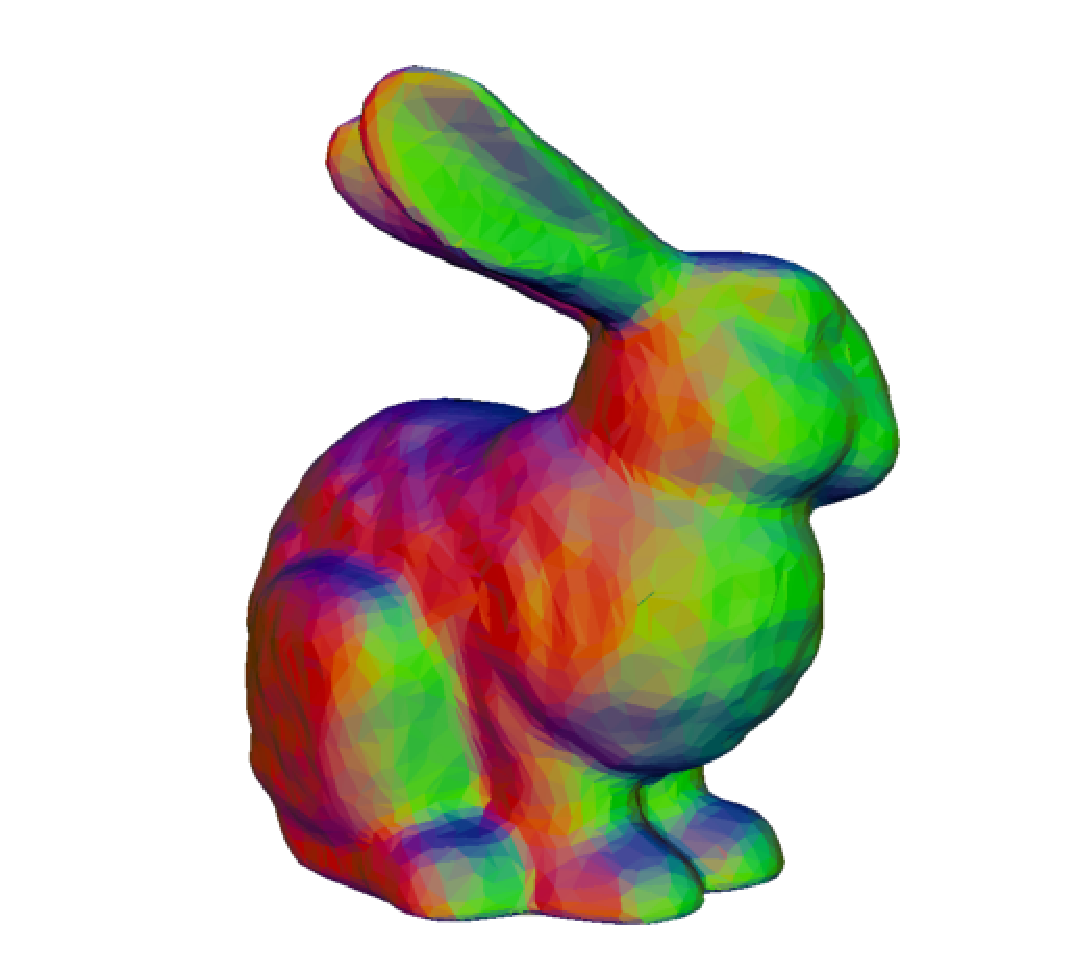
\includegraphics[scale=0.4]{bunny-normal.eps}}
  \subfloat[checker board, $L = 1.0$]{
    \label{fig:bunny-checker}
    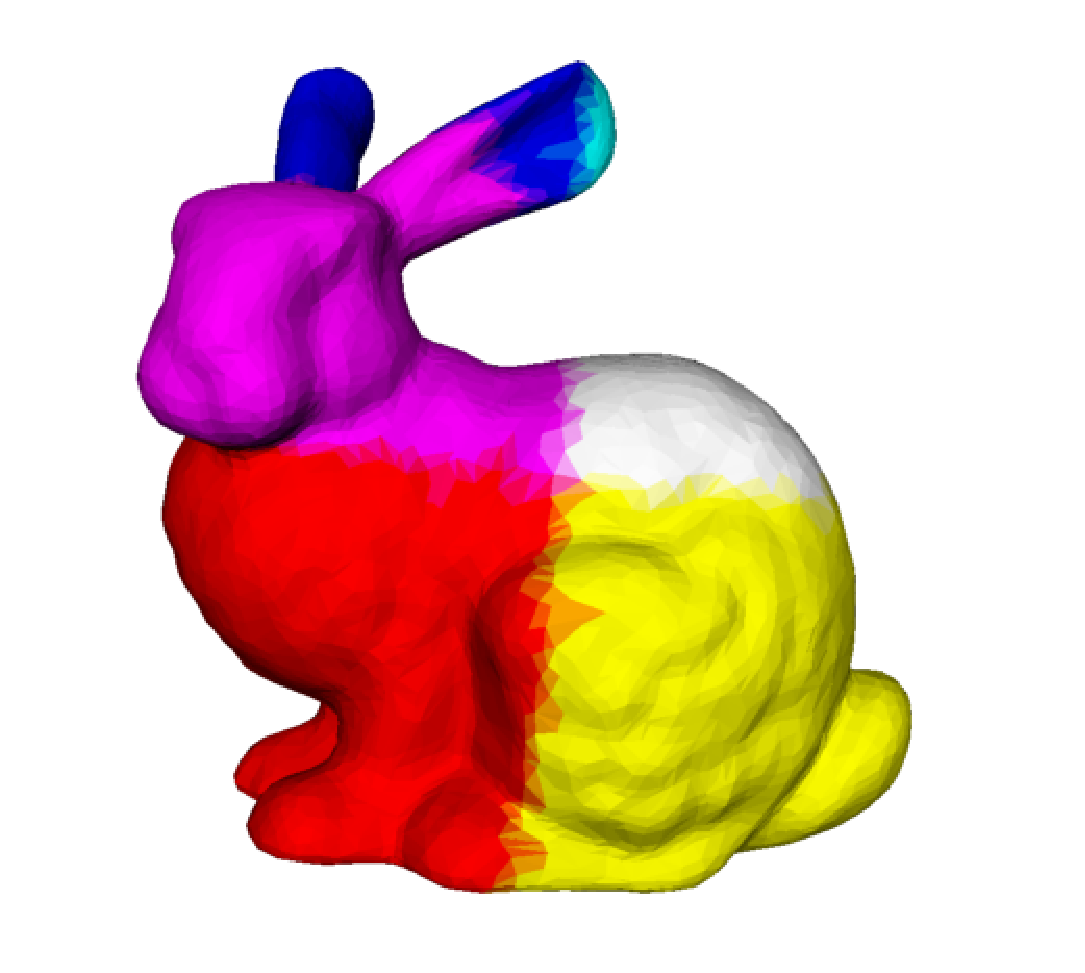
\includegraphics[scale=0.4]{bunny-checker-l1.eps}}

  \caption{Bunny}
\end{figure}

\begin{figure}
  \centering

  \subfloat[normal mapping]{
    \label{fig:feline-normal}
    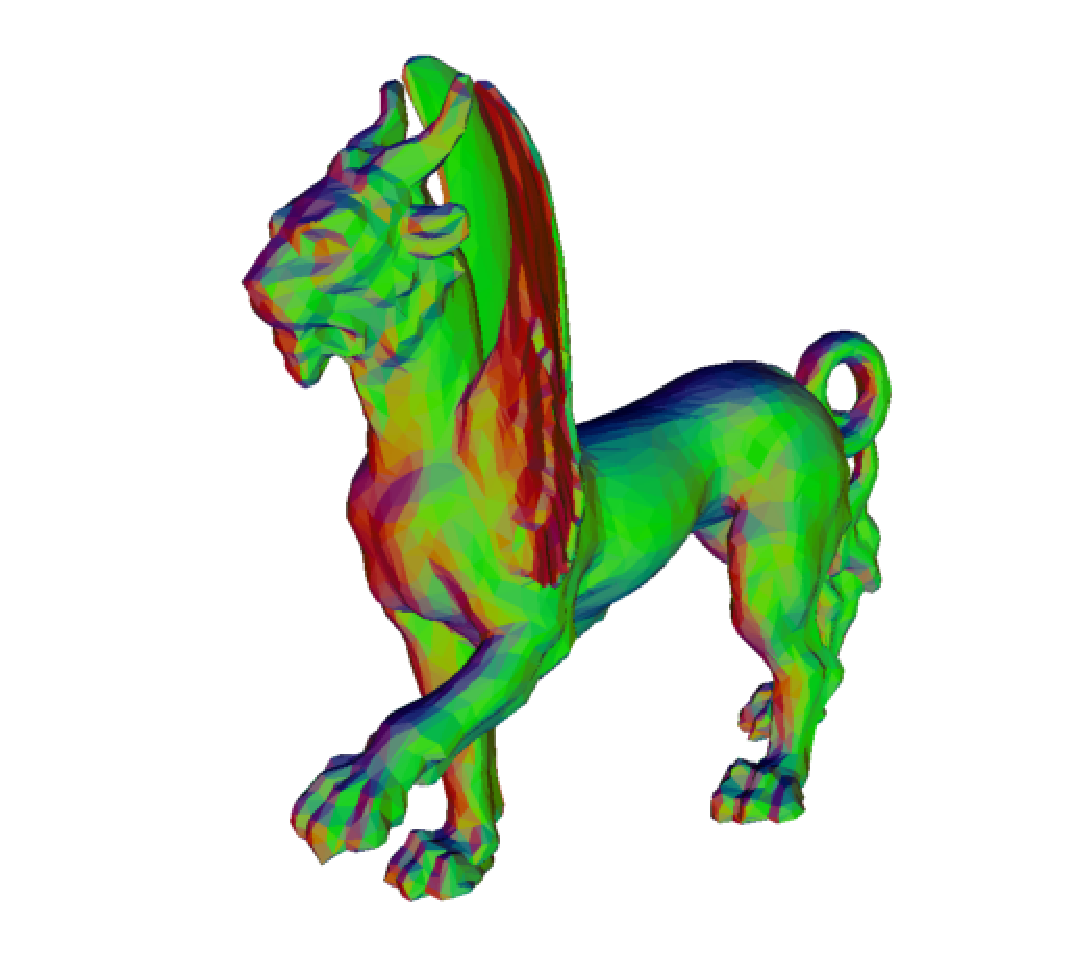
\includegraphics[scale=0.4]{feline-normal.eps}}
  \subfloat[checker board, $L = 0.5$]{
    \label{fig:feline-checker}
    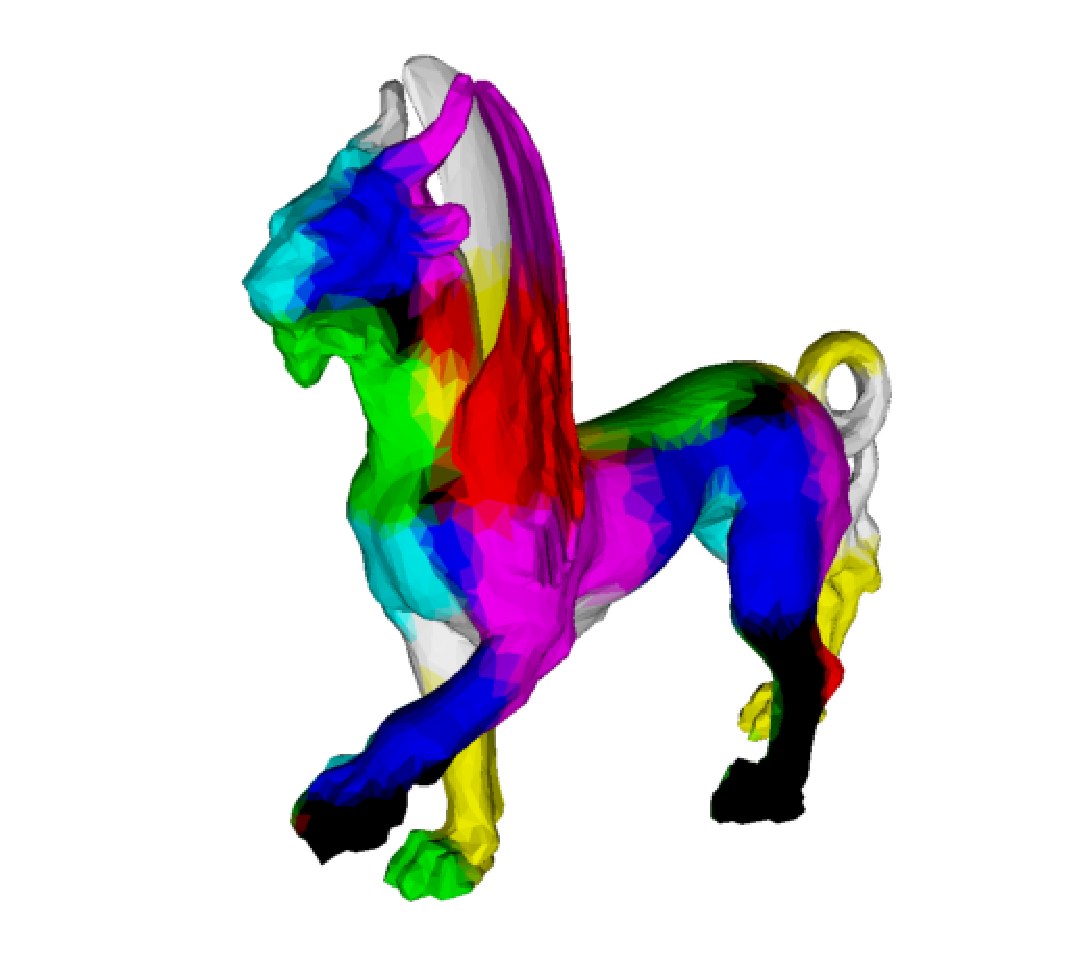
\includegraphics[scale=0.4]{feline-checker-l05.eps}}

  \caption{Feline}
\end{figure}

\begin{figure}
  \centering

  \subfloat[normal mapping]{
    \label{fig:buddha-normal}
    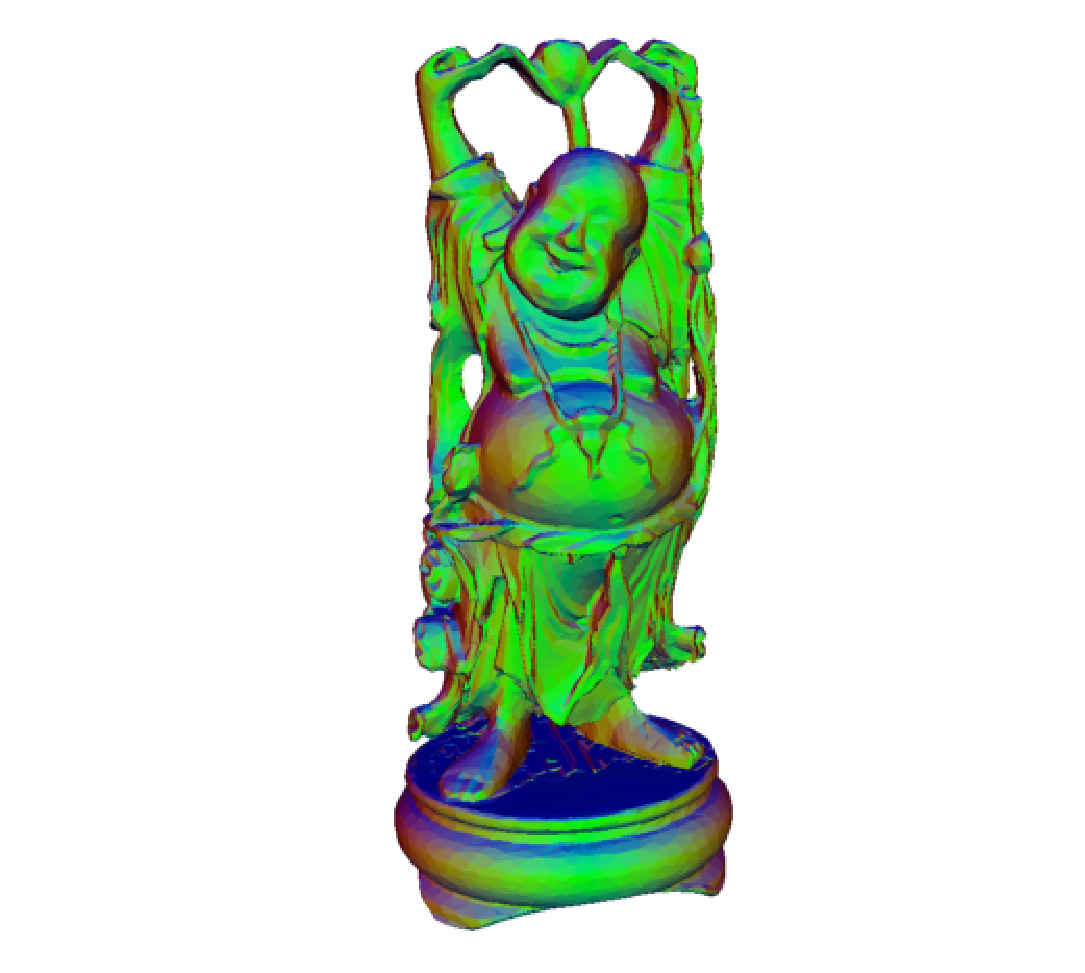
\includegraphics[scale=0.4]{buddha-normal.eps}}
  \subfloat[checker board, $L = 0.25$]{
    \label{fig:buddha-checker}
    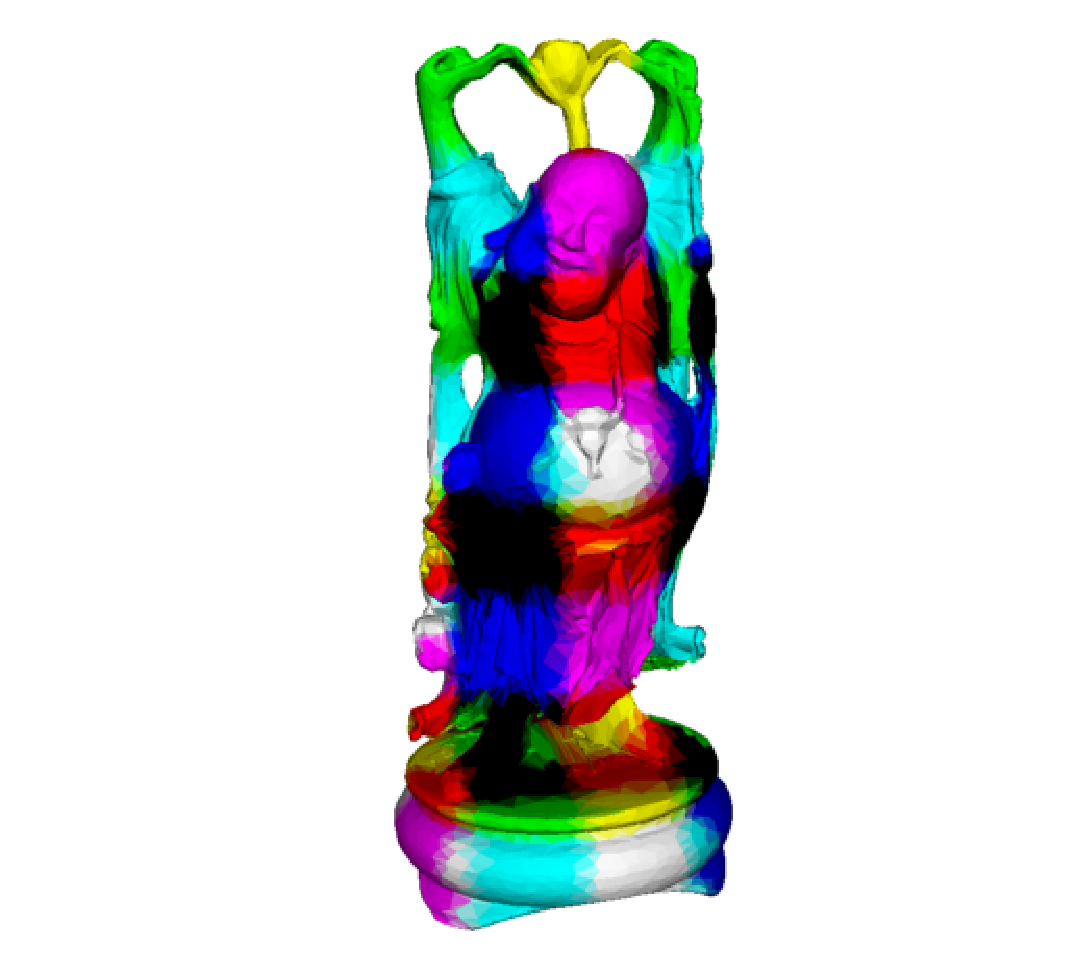
\includegraphics[scale=0.4]{buddha-checker-l025.eps}}

  \caption{Buddha}
\end{figure}

\begin{figure}
  \centering

  \subfloat[normal mapping]{
    \label{fig:dragon-normal}
    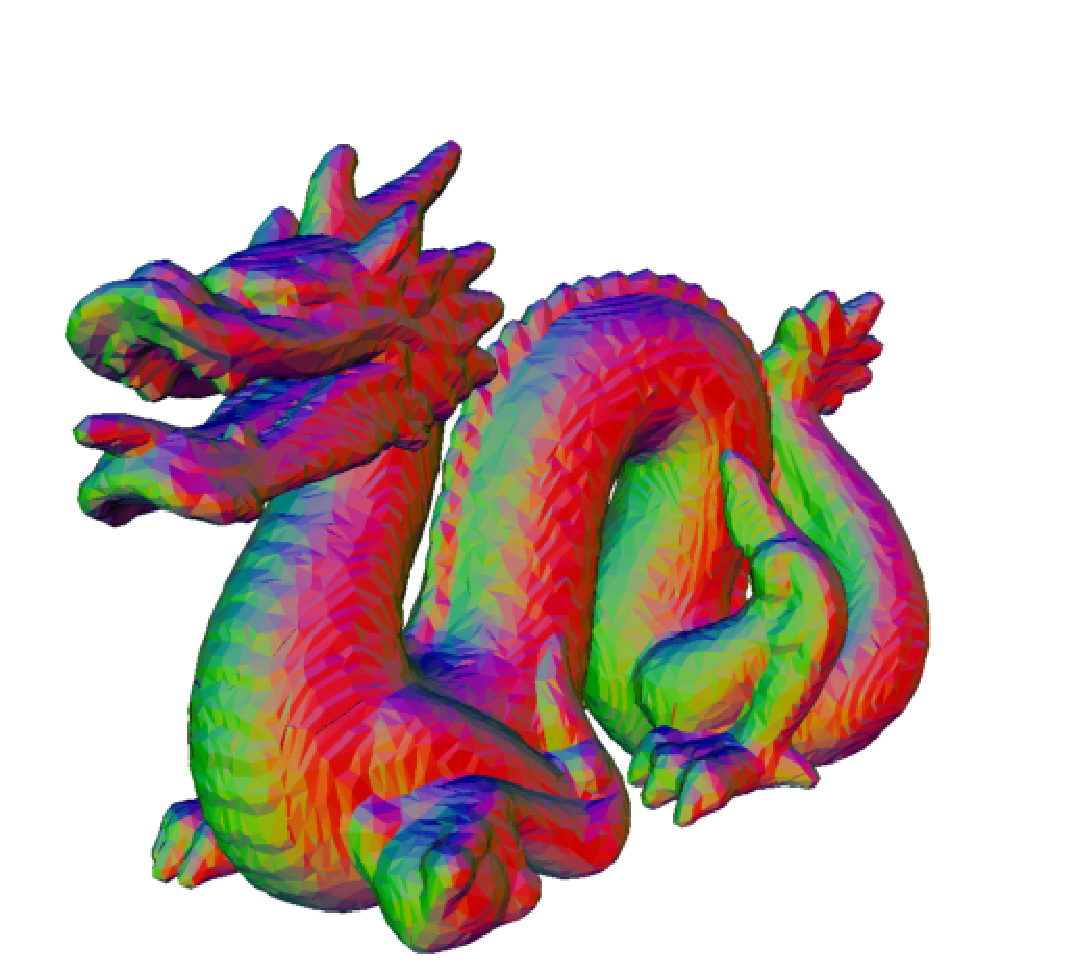
\includegraphics[scale=0.4]{dragon-normal.eps}}
  \subfloat[checker board, $L = 0.125$]{
    \label{fig:dragon-checker}
    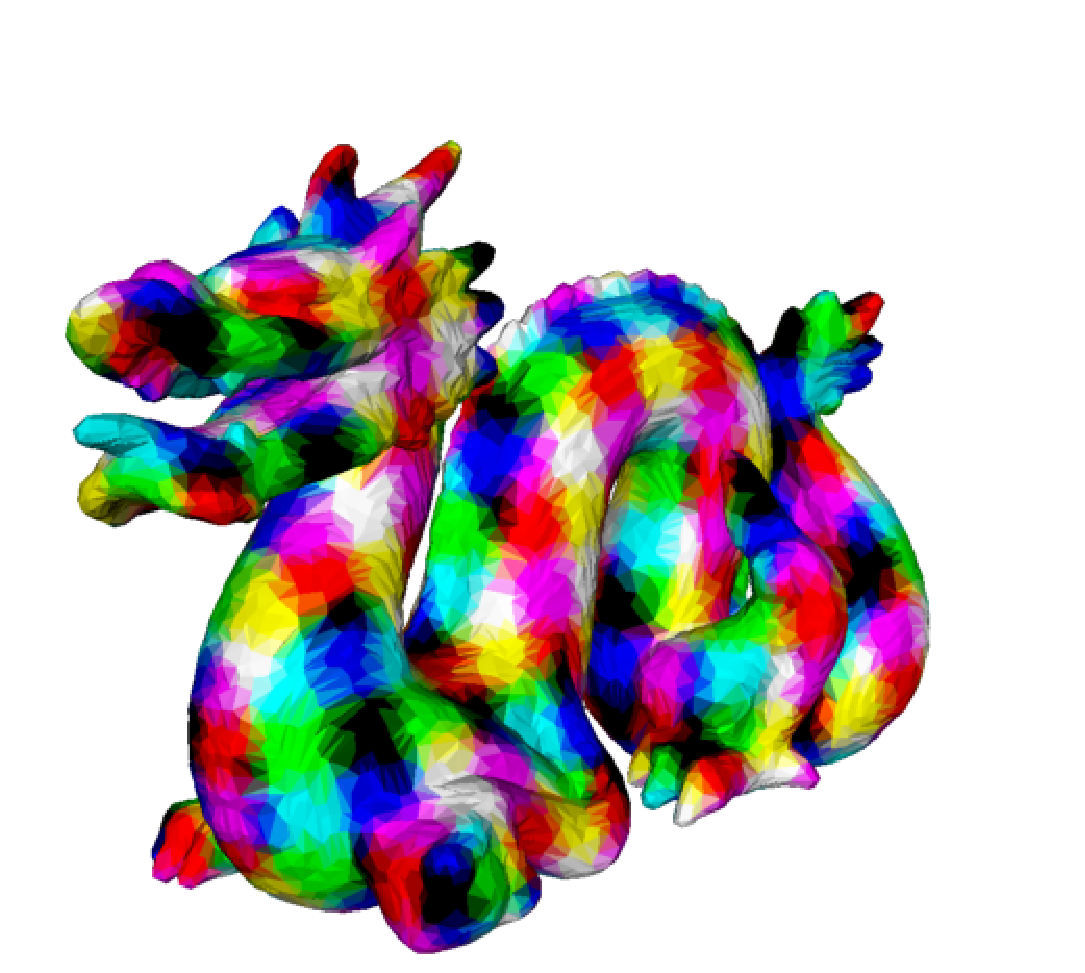
\includegraphics[scale=0.4]{dragon-checker-l0125.eps}}

  \caption{Dragon}
\end{figure}

\begin{figure}
  \centering

  \subfloat[checker board, $L = 0.5$]{
    \label{fig:icosahedron-checker1}
    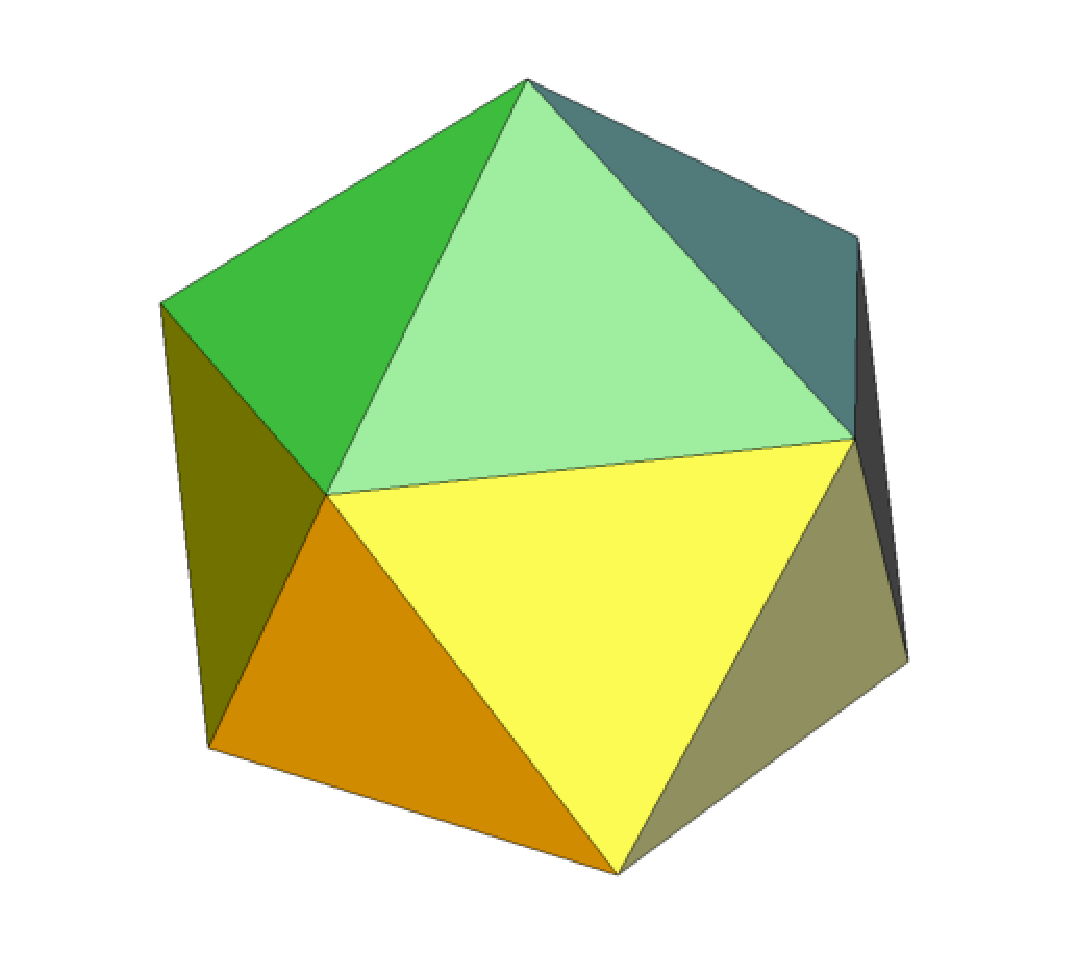
\includegraphics[scale=0.4]{icosahedron-checker-l05.eps}}
  \subfloat[checker board, $L = 1.0$]{
    \label{fig:icosahedron-checker2}
    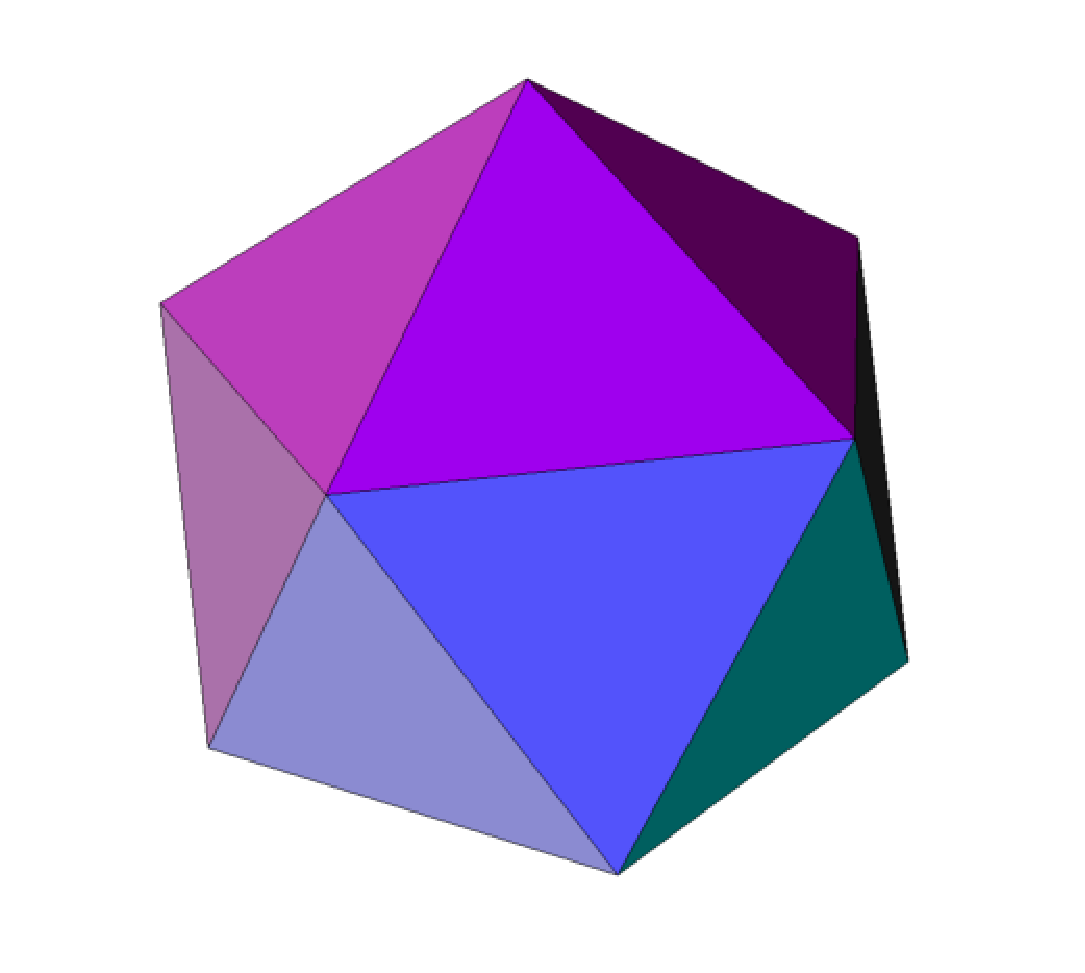
\includegraphics[scale=0.4]{icosahedron-checker-l1.eps}}

  \caption{Icosahedron}
\end{figure}

\pagebreak

\section{Polygon ID}

In this task we are asked to come up with a bijective mapping of an integer
polygon ID to some color. The task is a preparation for the following two and
is not required to give visually pleasing results, but should rather be simple.

For my solution I simply interpret the polygon ID $P$ as a base-$255$ number
with the RGB color components as coefficients:

\begin{equation}
 P = R \cdot 255^0 + G \cdot 255^1 + B \cdot 255^2 \qquad 0 \leq R,G,B \leq
255
 \label{eq:polygonid}
\end{equation}

This of course will only work for meshes with less than
$255+255^2+255^3=16646655$ polygons. Thankfully, this is the case for the
objects relevant to this exercise. As an additional restriction we reserve the
last color, i.e. white, to be used as the background color in the following two
exercises.

The results can be seen in fig. \ref{fig:bunny-polygonid},
\ref{fig:feline-polygonid}, \ref{fig:buddha-polygonid} and
\ref{fig:dragon-polygonid}. I was
surprised to see that the polygon IDs are apparently random and do not follow
any geometric route. As such, the colorization looks random as well, which can
be seen as an interesting side effect for this algorithm. If one tries to
create non-randomly sorted polygon IDs, he could verify whether he succeeded
easily by applying this colorization scheme.

The source code for this solution is located in
\texttt{Ex1\_2::setPolygonIdColors()}.

\begin{figure}
  \centering

 
  \subfloat[Bunny]{\label{fig:bunny-polygonid}
            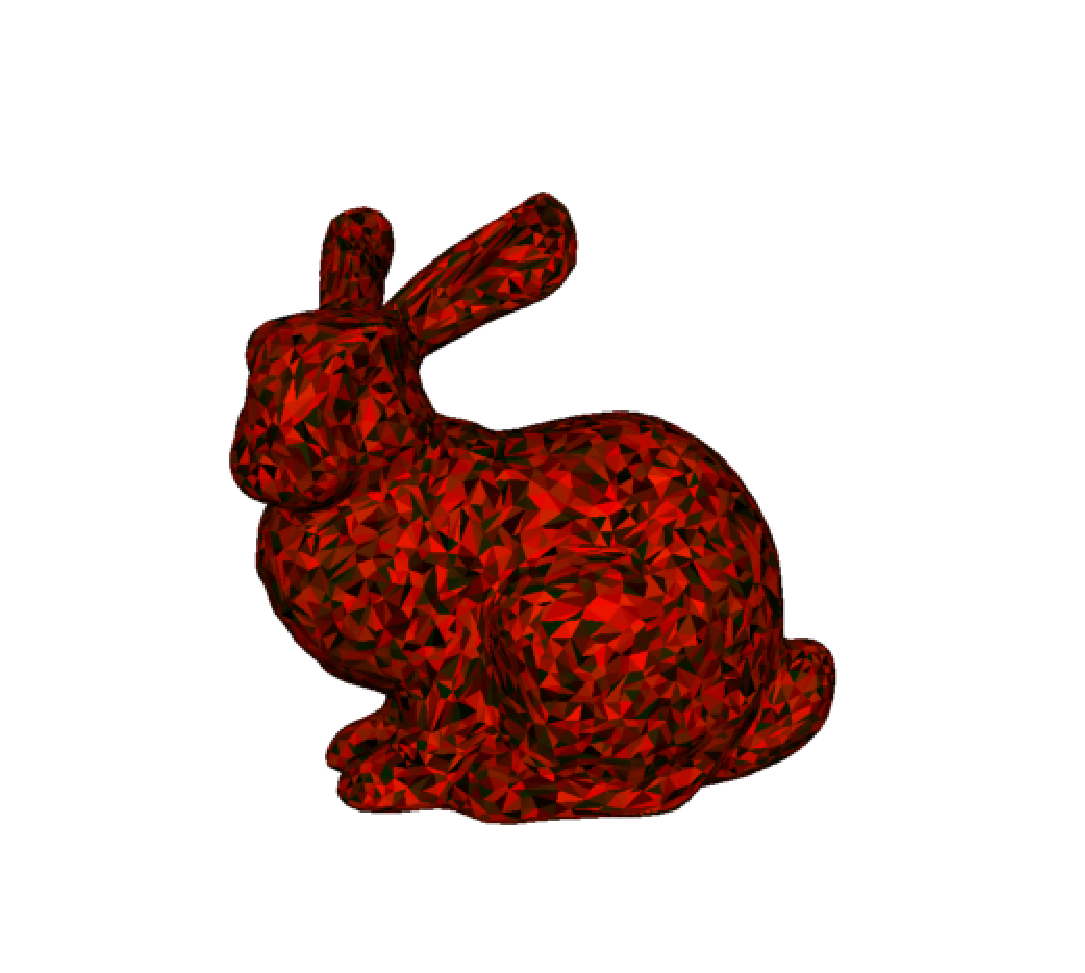
\includegraphics[scale=0.4]{bunny-polygonid.eps} }
  \subfloat[Feline]{\label{fig:feline-polygonid}
            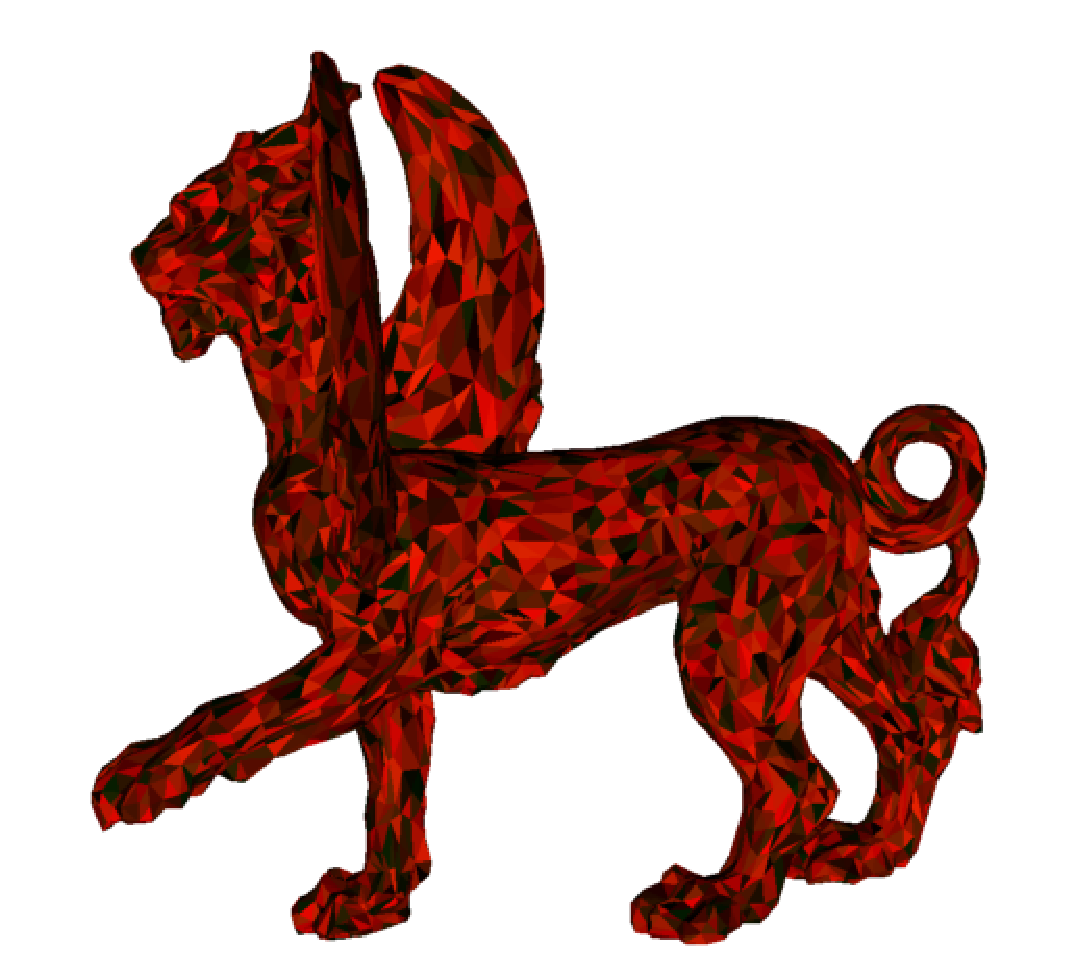
\includegraphics[scale=0.4]{feline-polygonid.eps} }
  \\
  \subfloat[Buddha]{\label{fig:buddha-polygonid}
            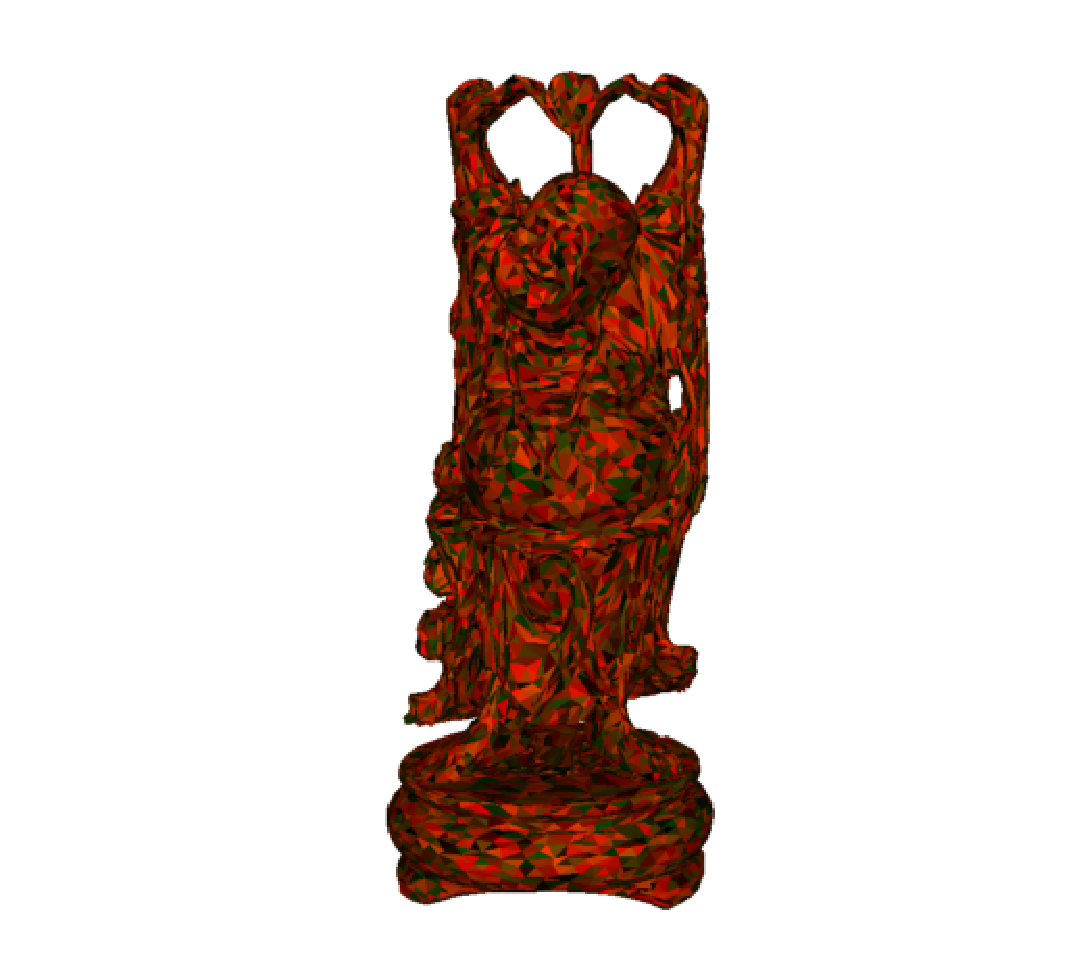
\includegraphics[scale=0.4]{buddha-polygonid.eps} }
  \subfloat[Dragon]{\label{fig:dragon-polygonid}
            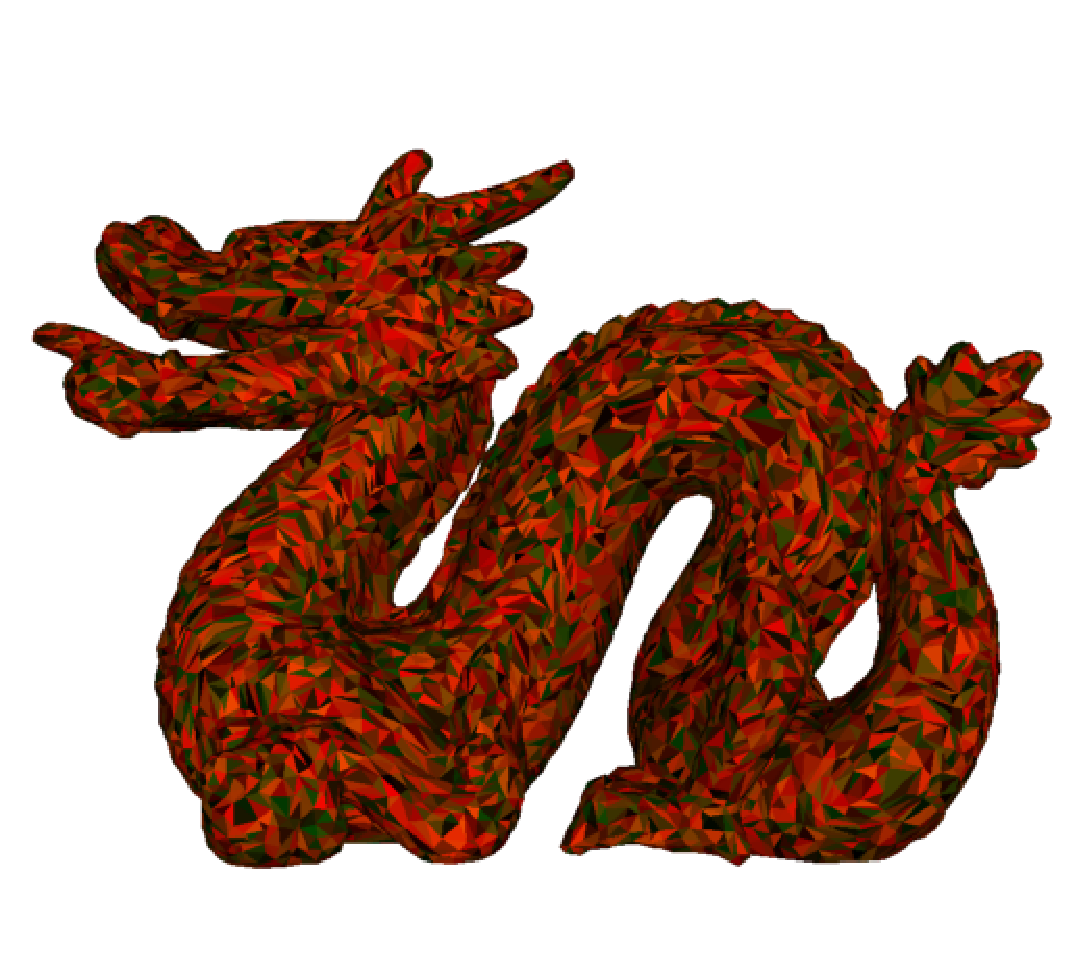
\includegraphics[scale=0.4]{dragon-polygonid.eps} }

  \caption{Polygon ID colorization}
\end{figure}

\pagebreak

\section{Surface Visibility}

This exercise was frustrating to say the least\dots Especially that we got the
hints on how to use the crude JavaView API just in the last week, made me waste
lots of time trying - and failing - to get something done for this exercise. I
deeply hope that this experience won't be repeated in future exercises.

The algorithm is simple to write down in textual form:

\begin{enumerate}
 \item apply Polygon ID colorization to geometry
 \item enclose geometry in sphere S
 \item iterate over vertices V of S
 \item rotate camera to point from V to center of geometry C
 \item render scene
 \item find unique set of colors in rendered scene
 \item map colors to polygon ID and increase counter for found IDs
 \item optionally weight by dot product of polygon normal and normalized view
vector
 \item continue for all vertices V of S 
 \item normalize result
\end{enumerate}

But as often when implementing a numerical algorithm, the problems lay in the
dirty details, like hitting the wall that is the JavaView-API\dots

\subsection{Enclosing Sphere}

Just one detail of the algorithm, yet one which took me quite some time to get
done. We are looking for a discretized sphere with at least 200 nodes.
Furthermore it should be as unbiased as possible, meaning the vertices should
be placed evenly on the sphere surface without favoring some areas, like the
poles.

\subsubsection{JavaView Sphere}

The obvious first choice was to use \texttt{PgElementSet::computeSphere(15,
15, r)} which wraps a plane of 225 vertices to a sphere. This mesh is biased
towards the poles though, where the node density is much larger compared to the
equator, as can be seen in fig. \ref{fig:grid-sphere}.

\begin{figure}
 \centering
 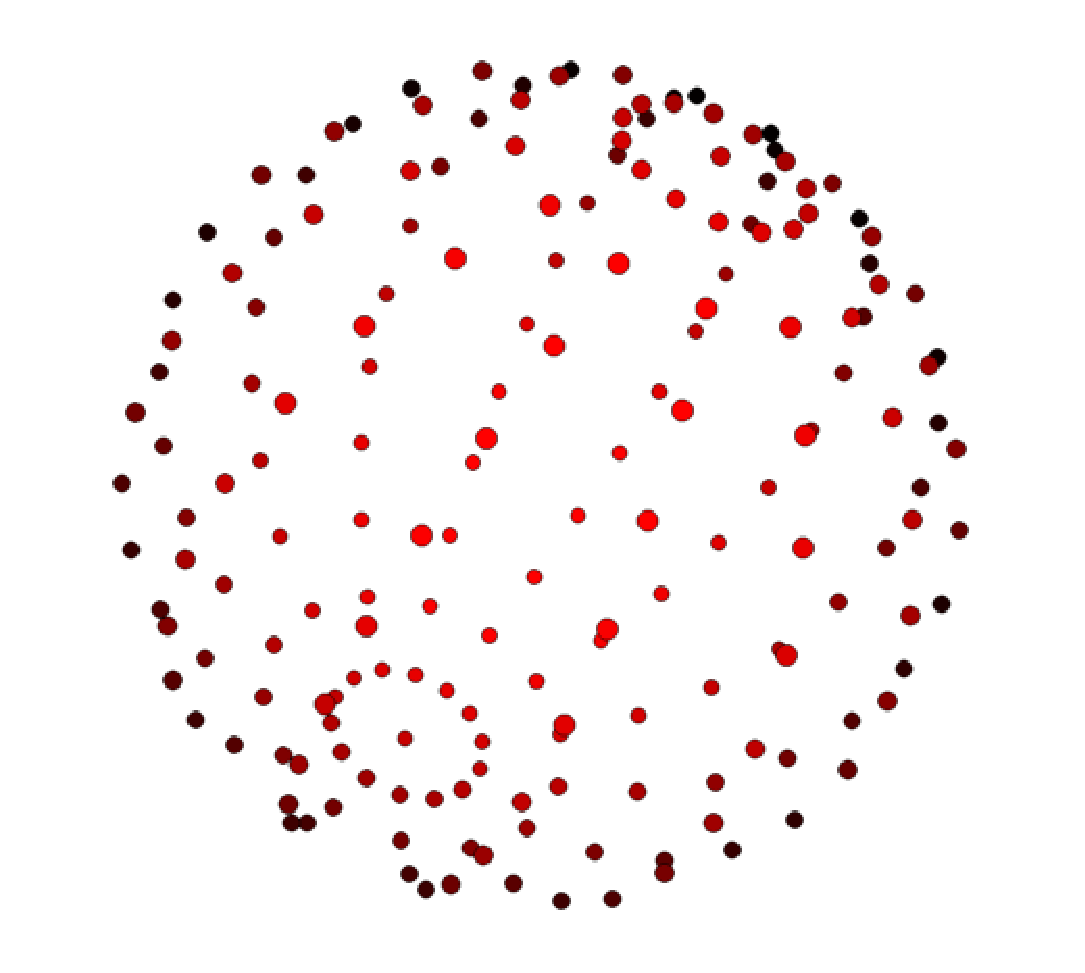
\includegraphics[scale=0.5]{sphere-grid.eps}
 \caption{Discretized sphere by wrapping a plane of 225 vertices}
 \label{fig:grid-sphere}
\end{figure}

\subsubsection{Subdivided Platonic Solid Take 1}

The exercise sheet suggests to take a platonic solid, e.g. an octahedron, and
apply a loop subdivision scheme. Sadly, the are no details given on how to do
this exactly, leaving me no choice but to try different alternatives.

As a first solution, I picked the aparrently simple route, by iteratively adding
vertices in the center $D$ of each polygon $ABC$. Then we subdivide the polygon
into three polygons $ABD$, $BCD$ and $ACD$. Since we are looking for a
discretized sphere, we have to scale $D$ such that its distance to the center of
the sphere equals the radius of our sphere.

While kind of straight forward to implement, it turned out that this approach
was not good: Since it only adds points in the middle of the polygons in each
step, the long edges from the initial octahedron will persist. This leads to an
uneven and hence biased distribution of the points on the sphere surface, which
can be seen in fig. \ref{fig:grid-platonic2}.

\begin{figure}
 \centering
 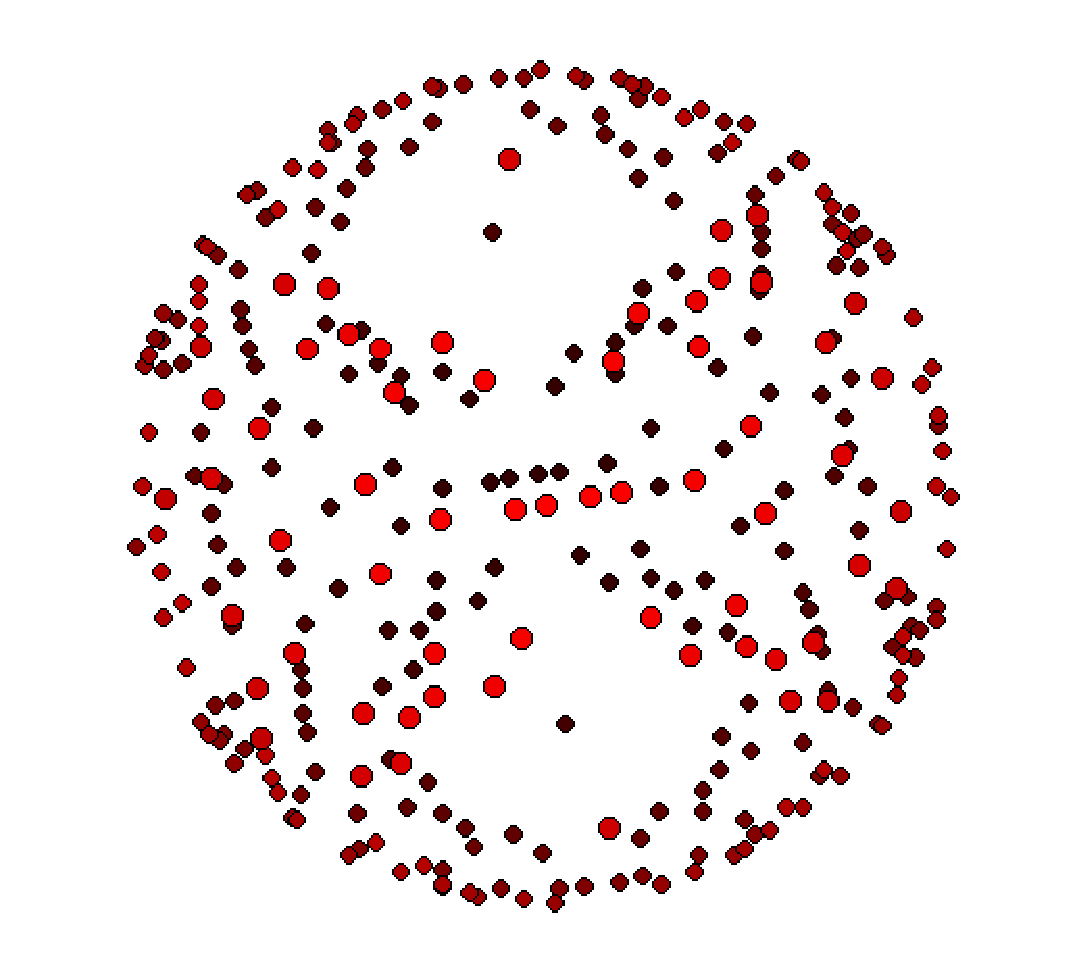
\includegraphics[scale=0.5]{platonic-1-grid.eps}
 \caption{Discretized sphere by iteratively subdeviding an Octohedron, adding
vertices in the center of each polygon in each step}
 \label{fig:grid-platonic2}
\end{figure}

\subsubsection{Subdivided Platonic Solid Take 2}

In my second approach I refined the previous algorithm by additionally adding
vertices in the middle of the edges of each polygon. Even though this sounds
rather simple, JavaView once again managed to make my life hard by preventing
me from iterating over the edges of an geometry\dots Anyhow, after some time I
got it working, as can be seen in \texttt{Ex1\_2::getViewPointsPlatonic()}.

Sadly, the result is also not optimal, resulting again in biased areas with
higher vertex density than others, as can be seen in fig.
\ref{fig:grid-platonic}. Another disadvantage is that the number of vertices
increases exponentially with each iteration step. As such it is no wonder that
we end up with a sphere of over 800 vertices, even though 200 are supposed to be
enough.

\begin{figure}
 \centering
 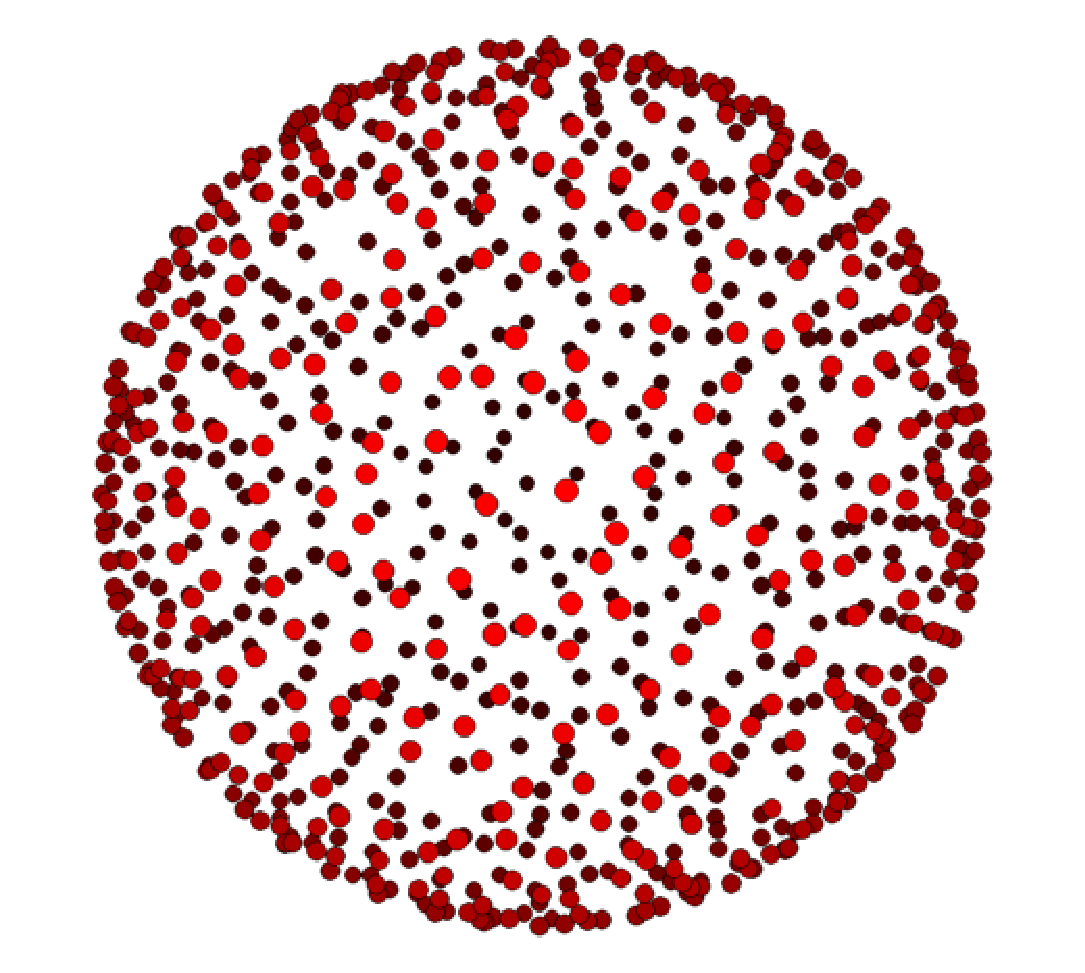
\includegraphics[scale=0.5]{platonic-grid.eps}
 \caption{Discretized sphere by iteratively subdeviding an Octohedron, adding
vertices in the center of each polygon and edge in each step}
 \label{fig:grid-platonic}
\end{figure}

\subsubsection{Sophe Grid}

Thus I resorted to another subdivision scheme I encountered during my
bachelors thesis: The XSophe Grid \cite{Hanson2004903}.
\texttt{Ex1\_2::getViewPoints()} shows how easy the implementation is. The
number of nodes in a thusly created mesh can be calculated via

\begin{equation}
 |V| = 2 + 8 \sum_{n=1}^N n - 4 N = 2 + 8 \cdot N/2 \cdot (N+1) - 4N = 2 + 4N^2.
\end{equation}

This equation is easy to understand: We have two points that represent the
south and north pole. The we sum the points per quarter hemisphere and multiply
it by 8. This way we count the points on the equator twice though, which is why
we substract them again.

In our case though we want to know $N$ for a given $|V| = 200$:

\begin{equation}
 N = \frac{\sqrt{|V| - 2}}{2}
\end{equation}

Besides being easy to implement and understant, the XSophe Grid also creates an
unbiased discretization of the sphere, as can be seen in fig.
\ref{fig:grid-sophe}. Due to these advantages, I decided to use this algorithm
for the calculation of the surface visibility.

\begin{figure}
 \centering
 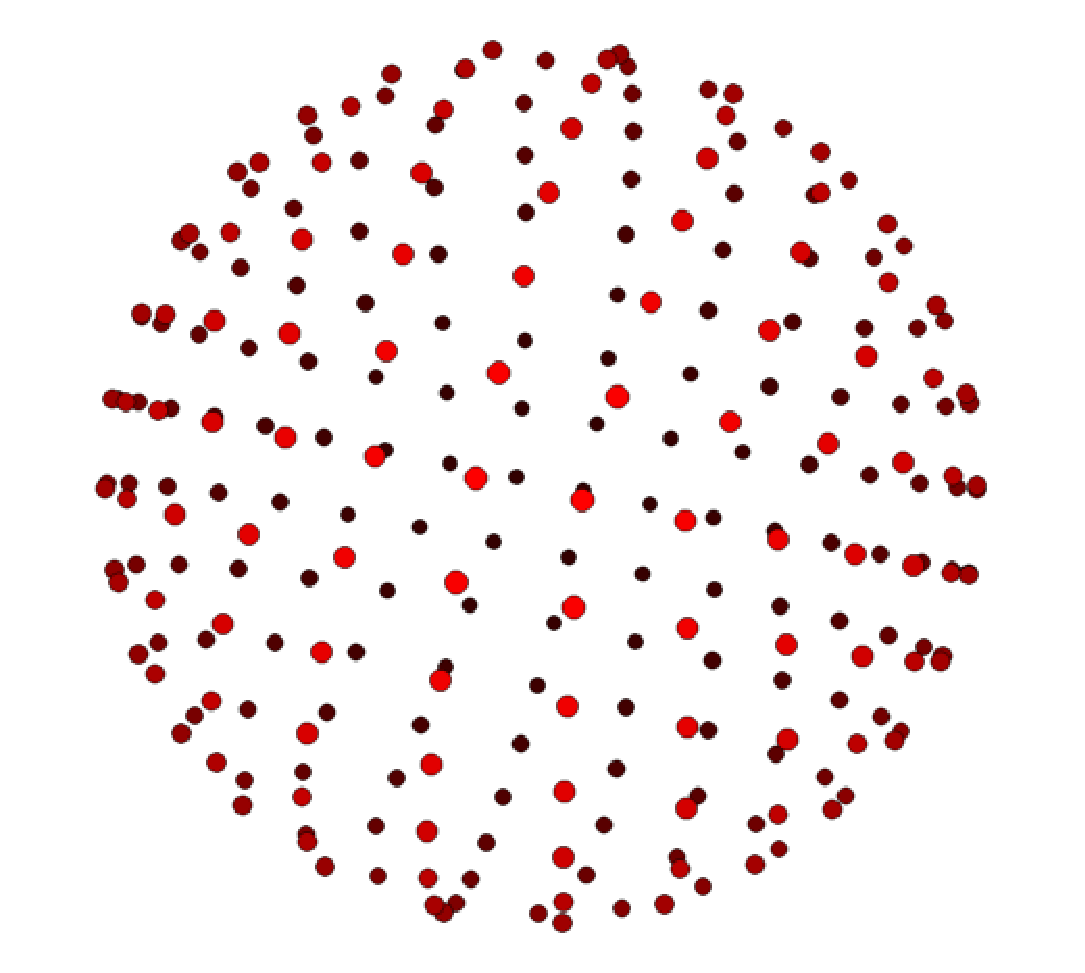
\includegraphics[scale=0.5]{sophe-grid.eps}
 \caption{Discretized Sphere following the Sophe Grid algorithm}
 \label{fig:grid-sophe}
\end{figure}

\subsubsection{Finding Visible Polygons}

Now we iterate over the vertices of the sphere and rotate our camera
accordingly. Then we let JavaView render the image into an offscreen buffer.
This part was again a huge waste of time due to the unintuitive API of JavaView
and was nearly impossible until we finally got the neccessary hints in the
recitation.

Once we have the image buffer though we simply have to iterate over all pixels
and read the image RGB color at this point. Using eq. \ref{eq:polygonid} we
directly get the associated polygon ID. We then find the unique list of colors
in the buffer and increase our counter for each of these.

For this all to work as expected though one must setup JavaView. Otherwise
unexpected colors might show up in the image, confusing the surface visibility
algorithm. For example one must register JavaView to prevent the ``missing
license'' warning text. Furthermore we must only paint elements with the special
\texttt{PvLightIf.MODEL\_SURFACE} lightning model set. Additionally antialiasing
must be disabled.

\subsubsection{Weighting and Normalization}

For the unweighted surface visibility we increase our counter by one for each
encountered color in each view point step. For normalization we then devide
these by the number of view points. As such the maximum surface visibility will
be 1, which can only occur though in the rare case of a single always
visible polygon.

If we are calculating the weighted surface visibility though, we increase the
counter not by one in each step, but by the projection of the polygon's normal
on the normalized view vector. The question then is how to normalize the final
counter values. The exercise only requests that the final maximum value will be
the same as in the unweighted surface visibility, i.e. 1. I decided to achieve
this by remembering the maximum projection value for each view point, then
deviding the counter values by the summed maximum projection values.

\subsubsection{Results}

The final results of my hours of work on the surface visibility are rather
unsatisfying. Especially for the icosahedron or sphere one expects equal
surface visibility for each polygon, which clearly is not the case as can be
seen in figures \ref{fig:sv-icosahedron} and \ref{fig:sv-sphere}.

For the larger models, like e.g. the dragon in fig. \ref{fig:sv-dragon}, the
results look rather random. Adjacent polygons get highly different surface
visibilities, which is rather bogus.

Comparing the weighted and unweighted surface visibility algorithms it is
obvious that my choice of normalization in the weighted case should be
improved. It turns out that it yields much lower absolute surface visibility
numbers which makes comparisons harder.

Additionally I find it noteworthy that the performance of both algorithms is
very bad. Especially the $O(n^2)$ algorithm for finding the colors in the
image buffer must be improved, as it is repeated for every view point. If one
could make JavaView paint to an image with an indexed colorspace of variable
size, with a direct getter for the used colors, the performance should be much
better. Sadly, I did not find any way to achieve this in Java.

\begin{figure}
 \subfloat[Unweighted]{
    \label{fig:usv-icosahedron}
    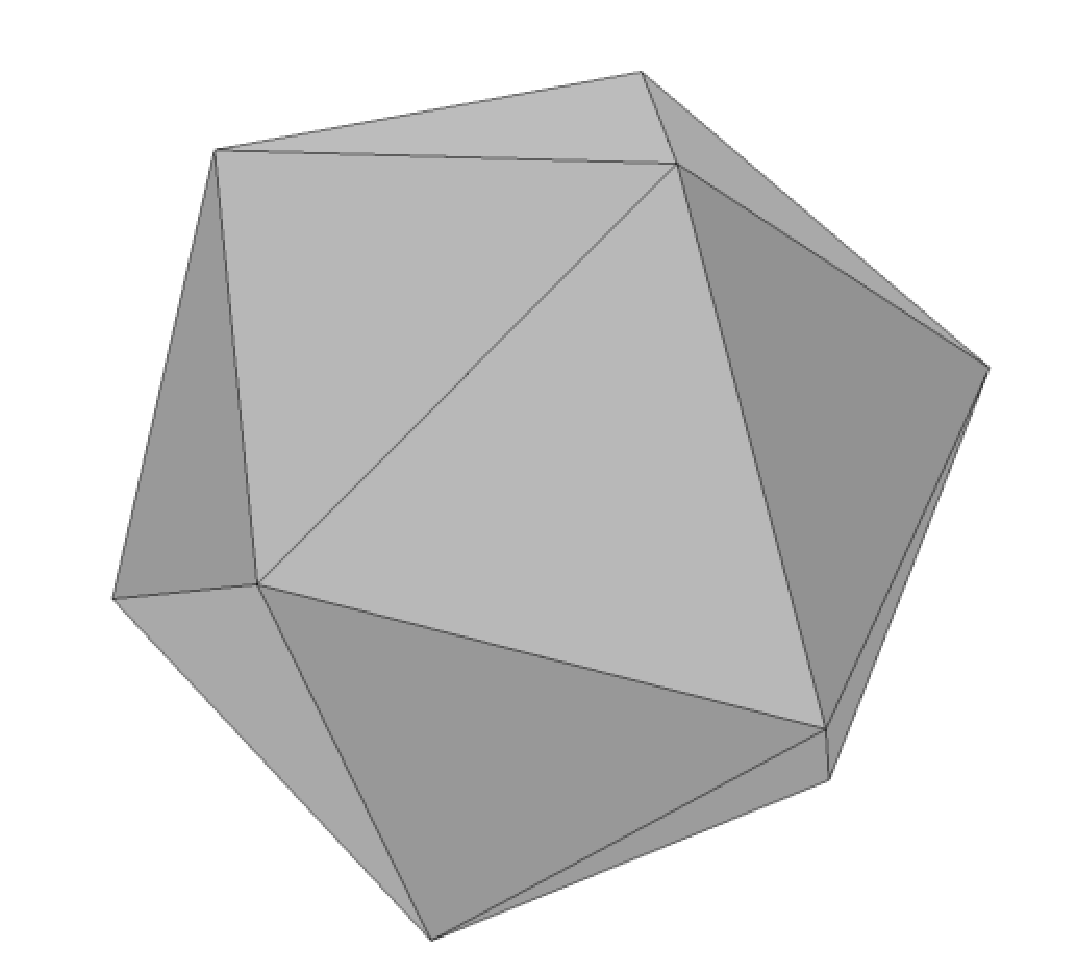
\includegraphics[scale=0.4]{usv-icosahedron.eps}}
 \subfloat[Weighted]{
    \label{fig:wsv-icosahedron}
    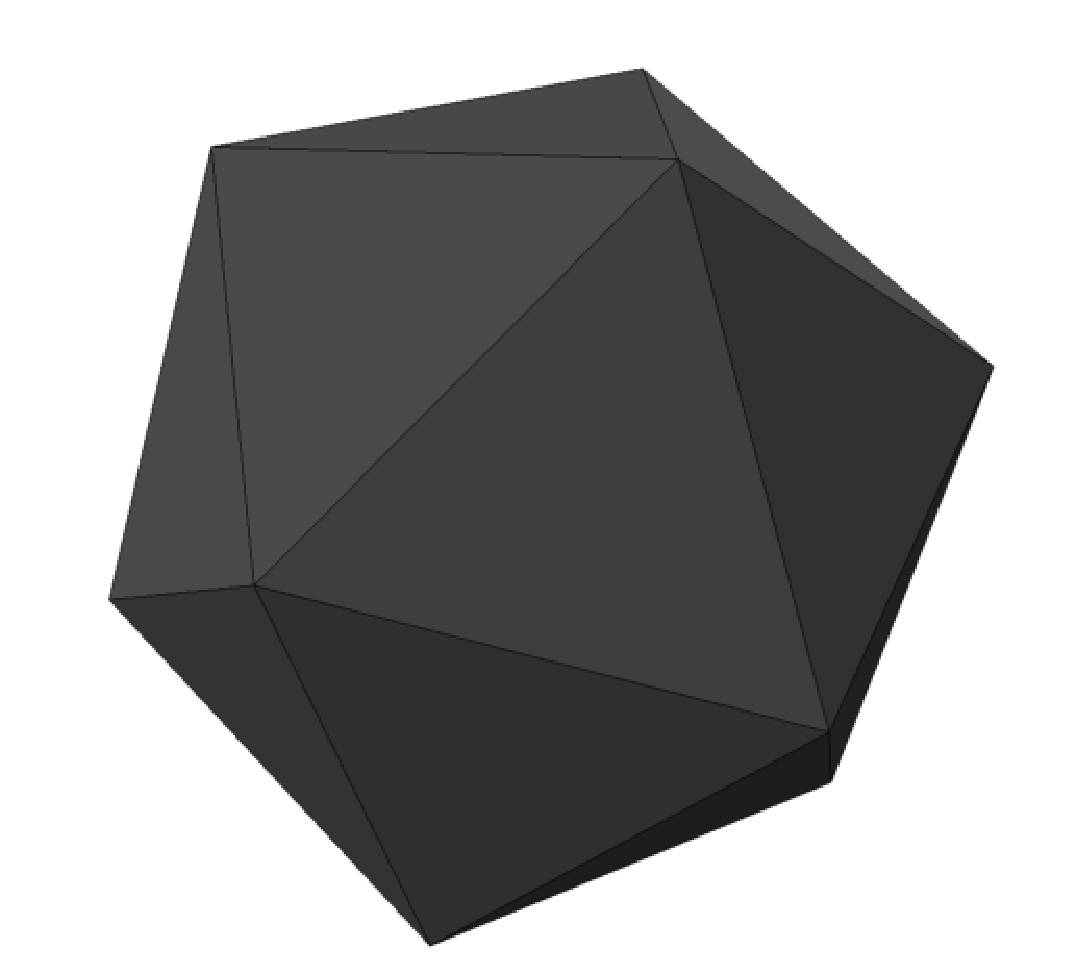
\includegraphics[scale=0.4]{wsv-icosahedron.eps}}
 \caption{Surface Visibility Calculation for the Icosahedron}
 \label{fig:sv-icosahedron}
\end{figure}

\begin{figure}
 \subfloat[Unweighted]{
    \label{fig:usv-sphere}
    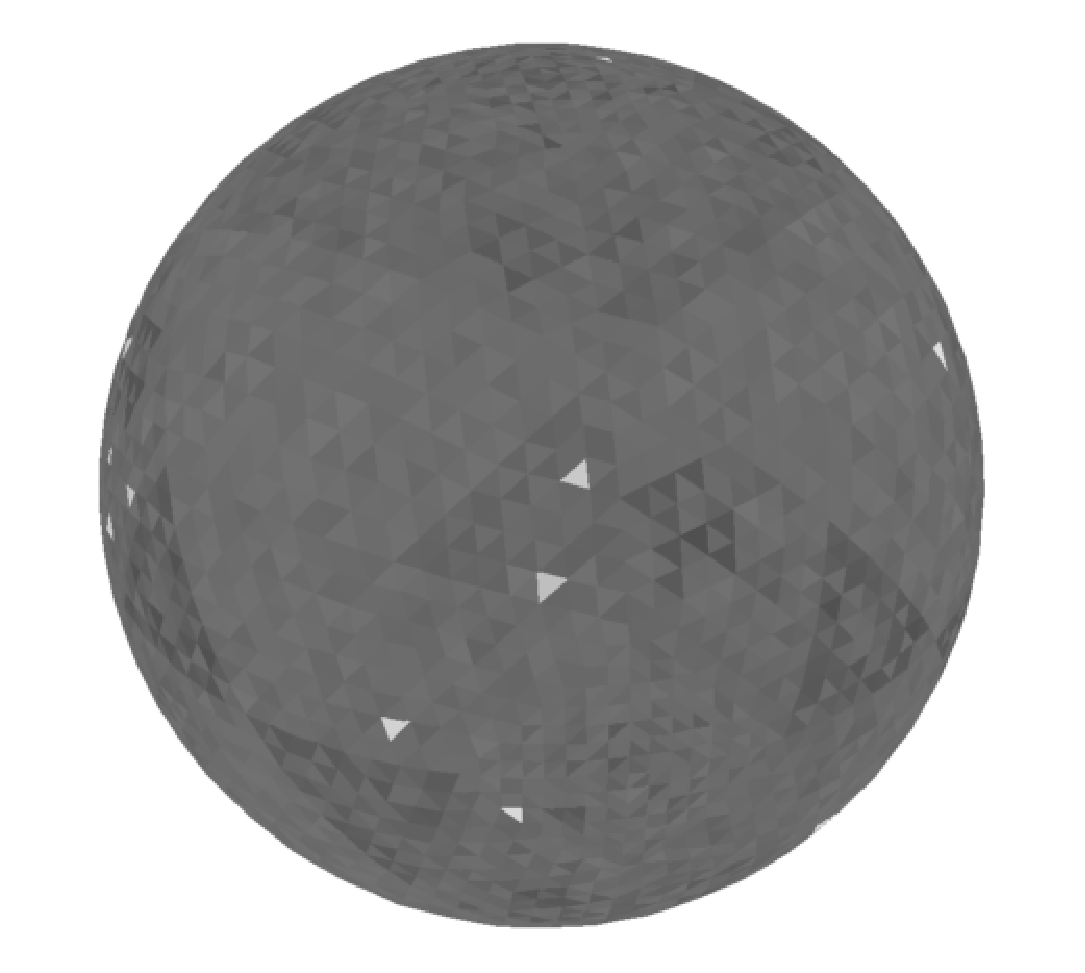
\includegraphics[scale=0.4]{usv-sphere.eps}}
 \subfloat[Weighted]{
    \label{fig:wsv-sphere}
    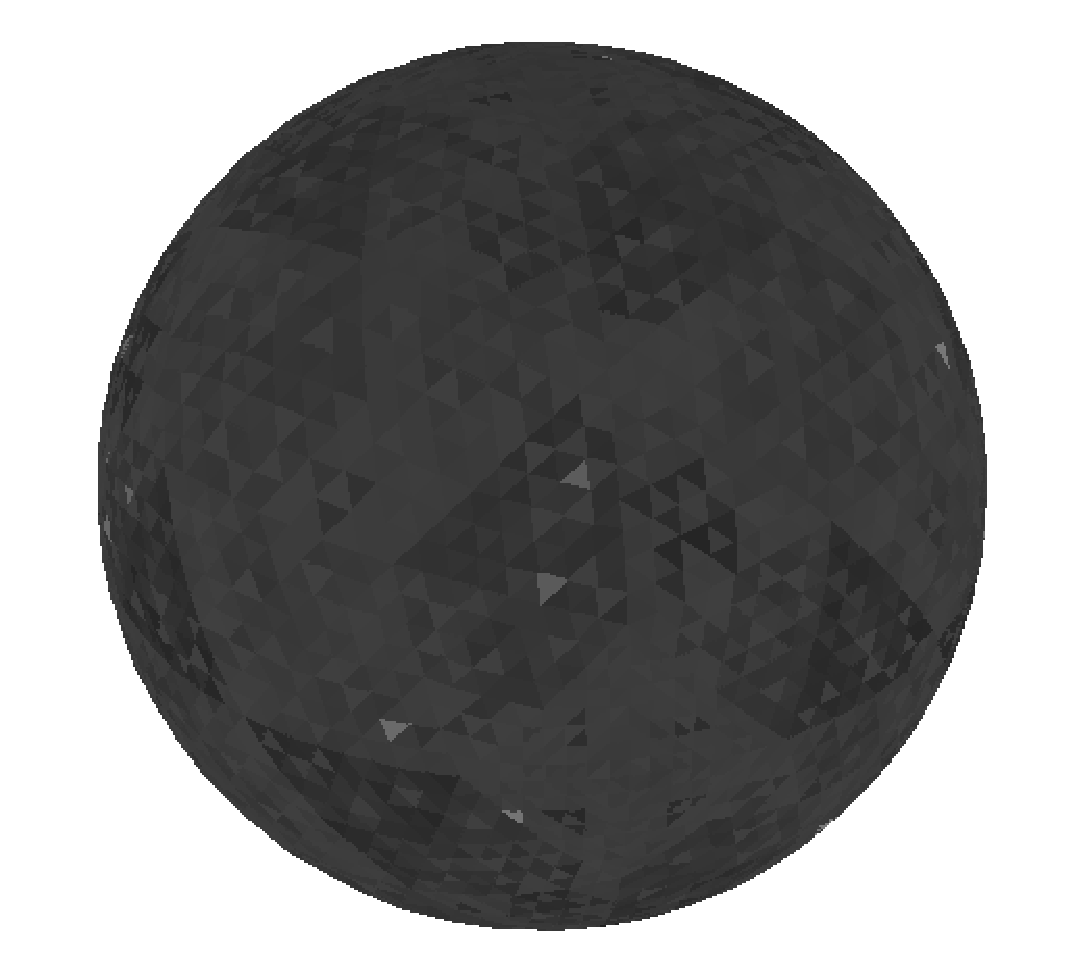
\includegraphics[scale=0.4]{wsv-sphere.eps}}
 \caption{Surface Visibility Calculation for the Sphere}
 \label{fig:sv-sphere}
\end{figure}

\begin{figure}
 \subfloat[Unweighted]{
    \label{fig:usv-dragon}
    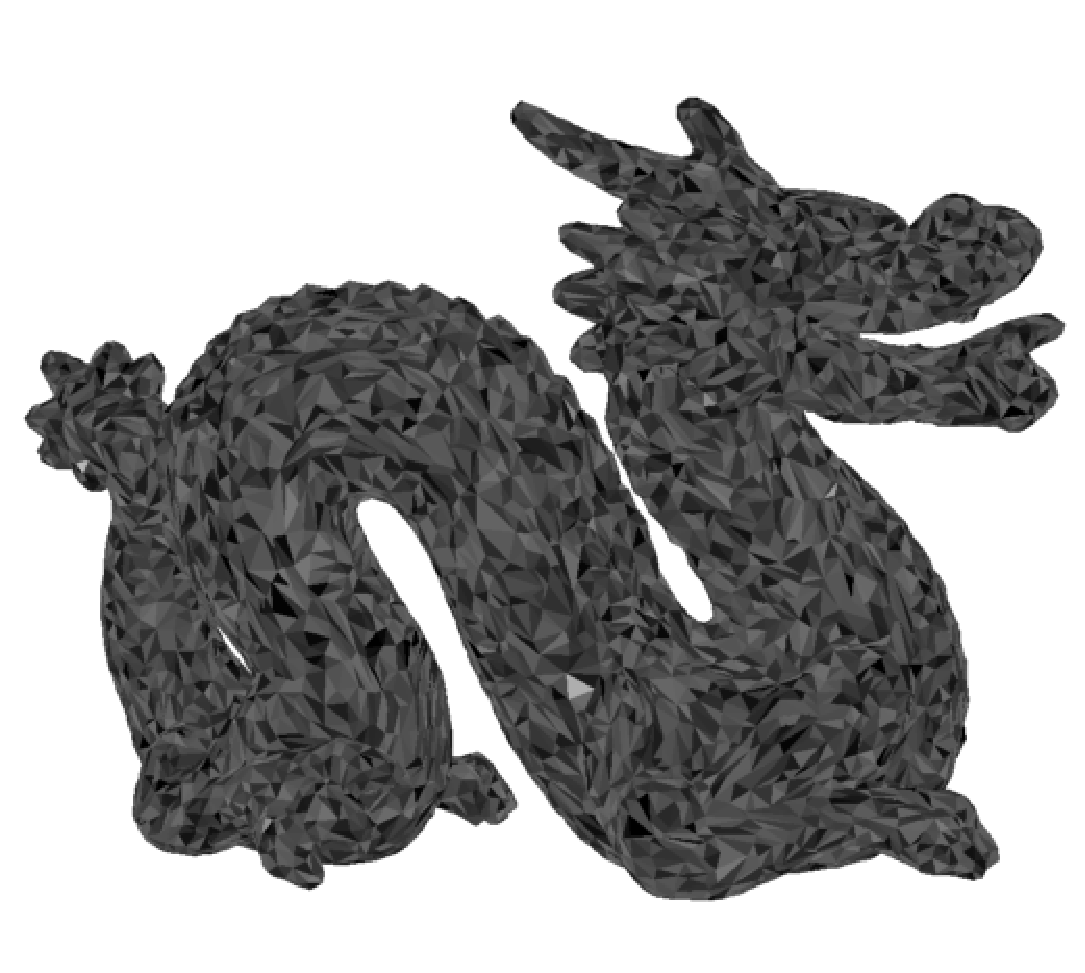
\includegraphics[scale=0.4]{usv-dragon.eps}}
 \subfloat[Weighted]{
    \label{fig:wsv-dragon}
    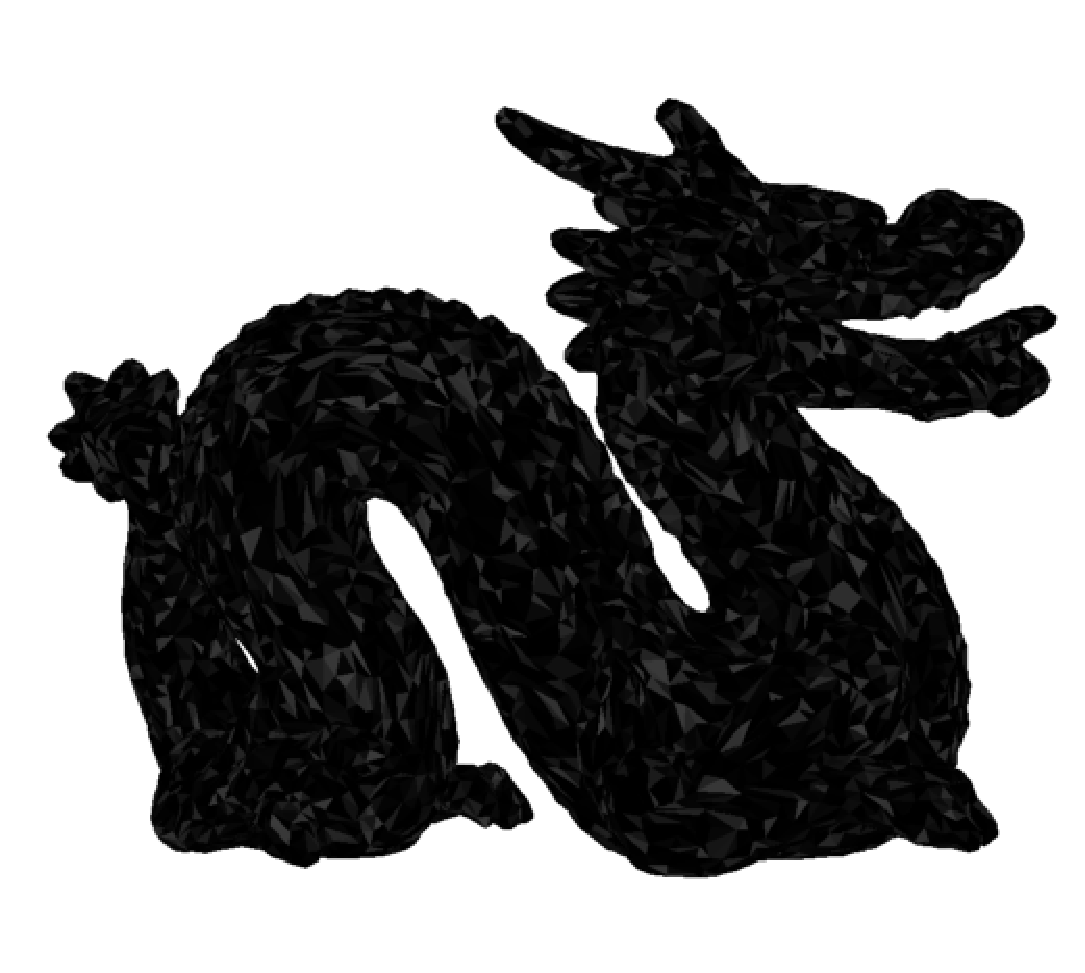
\includegraphics[scale=0.4]{wsv-dragon.eps}}
 \caption{Surface Visibility Calculation for the Dragon}
 \label{fig:sv-dragon}
\end{figure}

\bibliography{sources}

\end{document}

% kate: replace-tabs on;